\chapterimage{03_Polarizacija.jpg} % Chapter heading image

\chapter{Svetloba kot elektromagnetno valovanje}
V tem poglavju bomo prešli z geometrijskega  na valovni opis svetlobe in jo 
obravnavali kot elektromagnetno valovanje. Iz Maxwellovih enačb
bomo izpeljali valovno enačbo in poiskali njene rešitve.
Zapisali bomo energijski tok
in vpeljali polarizacijo elektromagnetnega valovanja. Na koncu
bomo zapisali še valovno enačbo v prevodni snovi in vpeljali 
kompleksni lomni količnik. 

\section{Valovna enačba v neprevodni snovi}
Obravnavajmo širjenje svetlobe po homogeni, izotropni in neprevodni snovi, 
v kateri ni prostih nabojev in električnih tokov. Na splošno elektromagnetno polje
opišemo z jakostjo  $\mathbf{E}$ in gostoto električnega polja $\mathbf{D}$\index{Jakost električnega polja}
\index{Gostota električnega polja}\index{Gostota magnetnega polja}\index{Jakost magnetnega polja}
ter gostoto $\mathbf{B}$ in jakostjo magnetnega polja $\mathbf{H}$. Te vektorske
količine med seboj niso neodvisne. Za količine električnega polja velja:
\begin{equation}
\mathbf{D} = \varepsilon \varepsilon_0 \mathbf{E},
\label{eq:DE}
\end{equation}
pri čemer sta $\varepsilon$ dielektričnost (ali tudi električna permitivnost)\index{Dielektričnost}
in $\varepsilon_0$
influenčna konstanta z vrednostjo $\varepsilon_0 = 8,85 \times 10^{-12}~\si{As/Vm}$. 
Med količinami magnetnega polja velja zveza:
\begin{equation}
\mathbf{H} = \frac{\mathbf{B}}{\mu \mu_0},
\label{eq:HB}
\end{equation}
pri čemer je $\mu$ magnetna permeabilnost,\index{Permeabilnost} konstanta $\mu_0$ pa je 
indukcijska konstanta z vrednostjo $\mu_0 = 4 \pi \times 10^{-7}~\si{Vs/Am}$.
Privzeli smo, da je snov izotropna, sicer bi morali $\varepsilon$ in $\mu$ pisati v 
tenzorski obliki. Prav tako smo privzeli, da so polja v snovi dovolj šibka, da
se snov odziva linearno. Nelinearen odziv, ki ga obravnava obširno področje
nelinearne optike, presega okvir te knjige.\footnote{~Glej npr. M. Čopič in M. Vilfan, 
{\it Fotonika}, Založba FMF, 2020.}

Količine električnega in magnetnega polja med seboj povezujejo Maxwellove
enačbe:\index{Maxwellove enačbe}
\boxeq{eq:Maxwell1}{
\nabla\times\mathbf{H} & =\frac{\partial\mathbf{D}}{\partial t}+\mathbf{j}_e,\\
\nabla\times\mathbf{E} & =-\frac{\partial\mathbf{B}}{\partial t}\label{eq:Maxwell2},\\
\nabla\cdot\mathbf{D} & =\varrho_{e}\label{eq:Maxwell3}, \\
\nabla\cdot\mathbf{B} & =0.\label{eq:Maxwell4}
}

Enačbe smo zaradi splošnosti zapisali v celotni obliki. Mi bomo 
obravnavali le primer, ko sta gostota električnega toka $\mathbf{j}_e$ in 
gostota prostih nabojev $\varrho_e$ enaki nič.\index{Amp\`{e}rov zakon}
\index{Faradayev zakon}\index{Gaussov zakon}\index{Gaussov zakon za magnetno polje}

\begin{remark}
Prvo od zapisanih Maxwellovih enačb imenujemo tudi Amp\`{e}rov zakon,
drugo Faradayev indukcijski zakon,
tretjo Gaussov zakon in četrto po analogiji Gaussov zakon za magnetno polje.
\end{remark}

Izhajamo iz enačbe~(\ref{eq:Maxwell2}) in na njej naredimo rotor:
\begin{equation}
\nabla \times \left(\nabla\times\mathbf{E}\right) =
\nabla \times \left(-\frac{\partial \mathbf{B}}{\partial t} \right)\!\!.
\label{eq:03_01}
\end{equation}
Levo stran enačbe preoblikujemo z upoštevanjem splošne zveze:
\begin{equation}
\nabla \times (\nabla \times \mathbf{E}) = \nabla (\nabla \cdot \mathbf{E}) - \nabla^2 \mathbf{E}.
\label{eq:03_02}
\end{equation}
Jakost električnega polja $\mathbf{E}$  v prvem členu na desni najprej  
izrazimo z $\mathbf{D}$ (enačba~\ref{eq:DE}), nato pa upoštevamo še Gaussov zakon 
(enačba~\ref{eq:Maxwell3}) ob odsotnosti prostih nabojev. Sledi:
\begin{equation}
\nabla (\nabla \cdot \mathbf{E}) - \nabla^2 \mathbf{E} = \nabla \left(\nabla \cdot 
\frac{\mathbf{D}}{\varepsilon \varepsilon_0}\right) - \nabla^2 \mathbf{E} = - \nabla^2 \mathbf{E}.
\label{eq:03_03}
\end{equation}
Na desni strani enačbe~(\ref{eq:03_01}) odvoda po kraju in času zamenjamo, 
saj sta neodvisna. Upoštevamo enačbo~(\ref{eq:HB}), Amp\`{e}rov zakon (enačba~\ref{eq:Maxwell1}) 
in zvezo (\ref{eq:DE}). Dobimo:
\begin{equation}
\nabla \times \left(-\frac{\partial \mathbf{B}}{\partial t} \right) = 
- \frac{\partial}{\partial t}\left(\mu \mu_0 \nabla
\times \mathbf{H}\right) = - \mu \mu_0 \frac{\partial}{\partial t}\frac{\partial \mathbf{D}}{\partial t}
 = -\varepsilon \varepsilon_0 \mu \mu_0 \frac{\partial^2 \mathbf{E}}{\partial t^2}.
\label{eq:03_04}
\end{equation}
Z izenačenjem enačb~(\ref{eq:03_03}) in (\ref{eq:03_04}) dobimo valovno enačbo:\index{Valovna enačba}
\boxeq{eq:valovnaE}{
\nabla^2\mathbf{E} - \varepsilon \varepsilon_0 \mu \mu_0 \frac{\partial^2 \mathbf{E}}{\partial t^2} = 0.
}
Ponovimo še zapis leve strani valovne enačbe s komponentami:
\begin{equation}
\nabla^2 \mathbf{E} =  
\left[\begin{array}{c}
        \frac{\partial^2E_x}{\partial x^2} + \frac{\partial^2E_x}{\partial y^2} + \frac{\partial^2E_x}{\partial z^2}\\
        \frac{\partial^2E_y}{\partial x^2} + \frac{\partial^2E_y}{\partial y^2} + \frac{\partial^2E_y}{\partial z^2} \\
        \frac{\partial^2E_z}{\partial x^2} + \frac{\partial^2E_z}{\partial y^2} + \frac{\partial^2E_z}{\partial z^2}
      \end{array}\right]\!\!.
\label{eq:03_05}
\end{equation}
Podobno izpeljemo tudi valovno enačbo za gostoto magnetnega polja:
\begin{equation}
\nabla^2\mathbf{B} - \varepsilon \varepsilon_0 \mu \mu_0 \frac{\partial^2 \mathbf{B}}{\partial t^2} = 0.
\label{eq:valovnaB}
\end{equation}
Naša naloga bo poiskati rešitvi valovnih enačb $\mathbf{E}(\mathbf{r},t)$
in $\mathbf{B}(\mathbf{r},t)$ kot funkciji kraja $\mathbf{r}$ in časa $t$ pri danih robnih pogojih.

\section{Ravno valovanje}\index{Ravno valovanje}\index{Sinusno valovanje|see{Ravno valovanje}}
Najpreprostejša rešitev valovne enačbe je sinusno potujoče valovanje, ki ga zapišemo
v obliki:
\boxeq{eq:ravnival}{
\mathbf{E}(\mathbf{r},t) = \mathbf{E}_0 \cos \left(\mathbf{k}\cdot \mathbf{r} - \omega t + \delta\right) = 
\Re\left(\mathbf{E}_0 e^{i\mathbf{k}\cdot \mathbf{r} - i\omega t + i\delta}\right)
}
in 
\begin{equation}
\mathbf{B}(\mathbf{r},t) = \mathbf{B}_0 \cos \left(\mathbf{k}\cdot \mathbf{r} - \omega t + \delta\right) = 
\Re\left(\mathbf{B}_0 e^{i\mathbf{k}\cdot \mathbf{r} - i\omega t + i\delta}\right)\!\!.
\label{eq:ravnivalB}
\end{equation}
Pri tem nastavku sta amplitudi valovanja $\mathbf{E}_0$ in $\mathbf{B}_0$ konstantni, 
$\mathbf{k}$ označuje valovni vektor,\index{Valovni vektor}\index{Krožna frekvenca}
$\omega$ krožno frekvenco in $\delta$ konstantno fazo\index{Faza valovanja}
valovanja.

Poglejmo naprej krajevno in časovno odvisnost zapisane rešitve. Če se zaradi nazornosti 
omejimo na valovanje, ki potuje v smeri $z$, sinusno valovanje, ki ga opisuje 
enačba~(\ref{eq:ravnival}) preprosto narišemo. Ob danem trenutku (pri izbranem $t$) je odvisnost 
velikosti jakosti električnega polja od koordinate sinusna in prikazana na sliki~\ref{fig:03_sinus}.  

Vpeljemo valovno dolžino valovanja $\lambda$ kot krajevno periodo sinusnega vala.\index{Valovna dolžina}
Zanjo velja zveza $k\lambda = 2\pi$, od koder izračunamo velikost valovnega vektorja oziroma 
valovno število $k$:\index{Valovno število}
\boxeq{eq:valovnivektor}{
k = \frac{2\pi}{\lambda}.
}
Podobno narišemo sinusno odvisnost od časa na danem mestu (pri izbranem $z$). 
Časovna perioda je $t_0$, namesto krožne frekvence $\omega$ pa pogosto uporabljamo 
frekvenco valovanja $\nu$:\index{Frekvenca valovanja} 
\boxeq{eq:freq}{
\nu = \frac{1}{t_0} = \frac{\omega}{2\pi}.
}
\begin{figure}[!h]
\centering
\def\svgwidth{90truemm} 
\input{slike/03_sinus.pdf_tex}
\caption{Spreminjanje velikosti jakosti električnega polja vzdolž smeri $z$ pri ravnem valovanju 
ob nekem trenutku.}
\label{fig:03_sinus}
\vglue-4truemm
\end{figure}

Vrnimo se k nastavku (enačba~\ref{eq:ravnival}) in fazo oziroma
argument kotne funkcije označimo s $\phi$:
\begin{equation}
\phi = \mathbf{k}\cdot \mathbf{r} - \omega t + \delta.
\label{eq:03_06}
\end{equation}
Ploskve konstantne faze dobimo pri konstantnem $\phi$. Ob danem trenutku velja:\index{Ploskev konstantne faze}\index{Valovna fronta|see{Ploskev konstantne faze}}
\begin{equation}
\mathbf{k}\cdot \mathbf{r} = \phi + \omega t - \delta = \mathrm{konst.}
\label{eq:03_08}
\end{equation}
Ta pogoj opisuje enačbo ravnine, pravokotne na vektor $\mathbf{k}$. Ploskve konstantne faze
oziroma valovne fronte so torej ravnine, ki so pravokotne na $\mathbf{k}$, žarki pa so premice, ki 
so vzporedne s $\mathbf{k}$ (slika~\ref{fig:03_ravnival}). Zapisana rešitev predstavlja ravno valovanje.
\begin{figure}[ht]
\centering
\def\svgwidth{90truemm} 
\input{slike/03_ravnival.pdf_tex}
\caption{Najpreprostejša rešitev valovne enačbe je ravno valovanje, pri katerem so ploskve konstante
faze (valovne fronte) ravnine, pravokotne na valovni vektor $\mathbf{k}$.}
\label{fig:03_ravnival}
\end{figure}
\vglue-5truemm
\begin{remark}
Jakost električnega polja je realna količina, kar je razvidno tudi iz zapisa (enačba~\ref{eq:ravnival}). 
V računih pogosto uporabljamo kompleksni zapis, to je brez omejitve na realni del. To lahko 
naredimo, dokler so jakosti polja majhne in velja linearna optika. Račun s kompleksnim zapisom
je navadno precej preglednejši in preprostejši, vendar moramo na koncu računa vedno vzeti le
realni del izračunane jakosti električnega polja. 
\end{remark}

\subsection*{Fazna hitrost}\index{Fazna hitrost}
Fazna hitrost je hitrost premikanja ploskev konstantne faze oziroma valovnih front. 
Če sledimo valovni fronti, je odvod faze $\phi$ po času konstanten in iz enačbe~(\ref{eq:03_06}) 
sledi:
\begin{equation}
\frac{d\phi}{dt}= \mathbf{k}\cdot \frac{d\mathbf{r}}{dt} - \omega = 0.
\label{eq:03_09}
\end{equation}
Zanima nas potovanje vzdolž smeri vektorja $\mathbf{k}$, 
zato lahko zapišemo $\mathbf{k}\cdot \mathbf{r} = kr$. Fazna hitrost, ki je določena 
s hitrostjo premikanja ploskev konstantne faze, je potem enaka:
\begin{equation}
v_f = \frac{dr}{dt} = \frac{\omega}{k}.
\label{eq:03_10}
\end{equation}
Poiščimo zvezo med $\omega$ in $k$ in izračunajmo fazno hitrost.

Vstavimo nastavek za ravno valovanje (enačba~\ref{eq:ravnival}) v valovno enačbo (enačba~\ref{eq:valovnaE}). 
Obravnavajmo zaenkrat samo eno komponento, na koncu bomo zapis razširili na tri komponente. 
Za komponento v smeri $x$ dobimo:
\begin{align}
\nabla^2E_x &= \frac{\partial^2E_x}{\partial x^2} + \frac{\partial^2E_x}{\partial y^2} + 
\frac{\partial^2E_x}{\partial z^2} \nonumber \\
&= \left(\frac{\partial^2}{\partial x^2} + 
\frac{\partial^2}{\partial y^2} + \frac{\partial^2}{\partial z^2}\right) \left(
E_{0x} \exp\left( ik_xx+ik_yy+ik_zz -i\omega t + i\delta\right) \right)\nonumber \\
&= \left( -k_x^2 -k_y^2-k_z^2\right) E_{0x} \exp\left( ik_xx+ik_yy+ik_zz -i\omega t + i\delta\right)\nonumber \\
&= -k^2 E_{0x} \exp\left( ik_xx+ik_yy+ik_zz -i\omega t + i\delta\right) = -k^2 E_x.
\label{eq:03_11}
\end{align}
Podoben izračun naredimo še za ostali komponenti in zapišemo Helmholtzevo enačbo:\index{Helmholtzeva enačba}
\begin{equation}
\nabla^2\mathbf{E}= -k^2 \mathbf{E}.
\label{eq:03_12}
\end{equation}
Odvajajmo nastavek (enačba~\ref{eq:ravnival}) še dvakrat po času:
\begin{equation}
\frac{\partial^2 \mathbf{E}}{\partial t^2} = - \omega^2 \mathbf{E}.
\label{eq:03_13}
\end{equation}
Iz valovne enačbe (enačba~\ref{eq:valovnaE}) tako dobimo zvezo:
\begin{equation}
-k^2 \mathbf{E} + \varepsilon\varepsilon_0\mu\mu_0 \omega^2 \mathbf{E} = 0
\quad \Longrightarrow \quad
k = \sqrt{\varepsilon\varepsilon_0\mu\mu_0}\,\omega.
\label{eq:03_15}
\end{equation}
Zdaj lahko zapišemo fazno hitrost (enačba~\ref{eq:03_10}):
\begin{equation}
v_f = \frac{\omega}{k} = \frac{1}{\sqrt{\varepsilon_0\mu_0}}\frac{1}{\varepsilon\mu}.
\label{eq:fazna}
\end{equation}
Kadar se elektromagnetno valovanje širi v praznem prostoru, sta $\varepsilon = 1$ in $\mu=1$. 
Hitrost elektromagnetnega valovanja -- in s tem tudi svetlobe --\index{Hitrost svetlobe}
v praznem prostoru označimo s $c_0$:
\boxeq{eq:c0}{
c_0 = \frac{1}{\sqrt{\varepsilon_0\mu_0}}.
}
V snovi je fazna hitrost potovanja svetlobe,\index{Hitrost svetlobe!{v dielektriku}}
ki jo navadno označujemo s $c$, manjša, in sicer:
\begin{equation}
c = v_f = \frac{c_0}{\sqrt{\varepsilon\mu}} = \frac{c_0}{n}.
\label{eq:03_16}
\end{equation}
Pri tem smo vpeljali lomni količnik snovi $n = \sqrt{\varepsilon\mu}$.\index{Lomni količnik} 
V optiki večinoma obravnavamo snovi, ki niso magnetne, zato je lomni količnik kar
enak korenu iz dielektričnosti:
\boxeq{eq:n}{
n = \sqrt{\varepsilon}.
}
\vglue-3truemm
\begin{remark}
Ne smemo pozabiti, da se dielektričnost s frekvenco elektromagnetnega 
valovanja spreminja. Pri izračunu lomnega količnika moramo zato upoštevati vrednost
dielektričnosti pri  frekvenci vidne svetlobe, kar je $\nu \sim 5 \times 10^{14}~\si{s}^{-1}$. 
\end{remark}

\begin{table}[ht]
 \centering
 \small
\begin{tabular}{|l|c||l|c|} \hline  
      Snov & $n$ & Snov & $n$ \\ \hline
      zrak & 1,00027 & glicerol & 1,47\\ \hline
      voda & 1,33 & steklo & 1,4 -- 1,9\\ \hline 
      led & 1,31 & safir & 1,77\\ \hline
      etanol & 1,36 & diamant & 2,42\\ 
\hline 
\end{tabular}
  \caption{Lomni količniki nekaterih izbranih snovi}
\label{table:n}
\end{table}

Vrnimo se k hitrosti svetlobe. Z upoštevanjem enačb~(\ref{eq:valovnivektor}) in (\ref{eq:freq})
izraz za $c$ preoblikujemo:
\begin{equation}
 c = \frac{\omega}{k} = \frac{2 \pi \nu}{2 \pi/\lambda}.
 \label{eq:03_17}
\end{equation}
Sledi:
\boxeq{eq:nulambda}{
c = \nu \lambda.
}
Produkt frekvence in valovne dolžine je torej enak fazni hitrosti svetlobe. Ker 
se v snovi hitrost svetlobe zmanjša, hkrati pa frekvenca ohranja, se 
v snovi zmanjša valovna dolžina valovanja. Če je v praznem prostoru valovna dolžina
$\lambda_0$, potem je v snovi z lomnim količnikom $n$ valovna dolžina enaka:
\begin{equation}
\lambda = \frac{\lambda_0}{n}.
\label{eq:03_18}
\end{equation}
\vglue-6truemm
\begin{remark}\index{Valovna dolžina}
Valovna dolžina vidne svetlobe v praznem prostoru sega od okoli $350~\si{nm}$, kar
vidimo kot temno vijolično barvo, do okoli $780~\si{nm}$, kar zaznamo kot temno rdečo 
barvo. Tem valovnim dolžinam ustrezajo frekvence od približno 
$4\times10^{14}~\si{s}^{-1}$ do približno $9\times10^{14}~\si{s}^{-1}$.
\end{remark}

\subsection*{Smeri vektorjev $\mathbf{E}$, $\mathbf{B}$ in $\mathbf{k}$}
Nadaljujmo z obravnavo elektromagnetnega valovanja v homogeni in izotropni snovi. 
Valovanje naj bo v obliki ravnega potujočega sinusnega valovanja, pri čemer se poslužimo praktičnega kompleksnega zapisa:
\begin{equation}
\mathbf{E}(\mathbf{r},t) = \mathbf{E}_0 e^{i\mathbf{k}\cdot \mathbf{r} - i\omega t + i\delta}
\qquad \mathrm{in} \qquad
\mathbf{B}(\mathbf{r},t) = \mathbf{B}_0 e^{i\mathbf{k}\cdot \mathbf{r} - i\omega t + i\delta}.
\label{eq:ravnivalkompleks}
\end{equation}
Izhajamo iz Gaussovega zakona (enačba~\ref{eq:Maxwell3}) in upoštevamo zvezo med 
$\mathbf{D}$ in $\mathbf{E}$ (enačba~\ref{eq:DE}): 
\begin{equation}
\nabla \cdot \mathbf{D} = \nabla \cdot \left( \varepsilon \varepsilon_0 \mathbf{E}\right) 
= \varepsilon \varepsilon_0 \left(\nabla \cdot \mathbf{E} \right)\!.
\label{eq:03_20}
\end{equation}
Iz tega sledi, da je ob odsotnosti prostih nabojev ($\varrho_{e} = 0$) divergenca 
jakosti električnega polja v izotropni snovi enaka nič.
Zapišemo jo kot:
\begin{align}
\nabla \cdot \mathbf{E} = \frac{\partial E_x}{\partial x}+ \frac{\partial E_y}{\partial y}+
\frac{\partial E_z}{\partial z} &= \left(ik_xE_{0x} + ik_yE_{0y} + ik_zE_{0z}\right)
e^{i\mathbf{k}\cdot \mathbf{r} - i\omega t + i\delta}\nonumber\\
&= i \left( \mathbf{E}_0 \cdot \mathbf{k} \right) e^{i\mathbf{k}\cdot \mathbf{r} - i\omega t + i\delta} = 
i\, \mathbf{E} \cdot \mathbf{k} = 0.
\label{eq:03_21}
\end{align}
Skalarni produkt jakosti električnega polja in valovnega vektorja je enak nič, kadar je:\index{Jakost električnega polja}
\boxeq{eq:Ekperp}{
\mathbf{E} \perp \mathbf{k}.
}
Na enak način iz enačbe~(\ref{eq:Maxwell4}) izpeljemo zvezo:\index{Gostota magnetnega polja}
\boxeq{eq:Bkperp}{
\mathbf{B}\perp \mathbf{k}.
}
Elektromagnetno valovanje je torej v izotropni snovi transverzalno, saj sta jakost
električnega in gostota magnetnega polja pravokotni na smer širjenja svetlobe.

Poiščimo še kot med $\mathbf{E}$ in $\mathbf{B}$. Ponovno izhajamo iz Maxwellove 
enačbe, tokrat iz Faradayevega zakona (enačba~\ref{eq:Maxwell2}). Magnetno polje ravnega valovanja 
odvajamo po času in dobimo zvezo:
\begin{equation}
\nabla\times\mathbf{E} = i \omega \mathbf{B}.
\label{eq:03_22}
\end{equation}
Nato izračunamo rotor jakosti električnega polja:
\begin{equation}
\nabla \times \mathbf{E} = 
\left|
\begin{array}{ccc}
\mathbf{e}_x & \mathbf{e}_y & \mathbf{e}_z\\
\frac{\partial}{\partial x} & \frac{\partial}{\partial y} & \frac{\partial}{\partial z}\\
E_{x} & E_{y} & E_{z}
\end{array}\right|
= 
\left[
\begin{array}{c}
ik_y E_z-ik_zE_y\\
ik_z E_x-ik_xE_z\\
ik_x E_y-ik_yE_x
\end{array}\right] = 
i\, \mathbf{k}\times \mathbf{E}.
\label{eq:03_23}
\end{equation}
Rezultat vstavimo v enačbo~(\ref{eq:03_22}) in dobimo:
\begin{equation}
\mathbf{k}\times \mathbf{E} = \omega \mathbf{B}.
\label{eq:EkB}
\end{equation}
Sledi ortogonalnost jakosti električnega $\mathbf{E}$ in gostote magnetnega
polja $\mathbf{B}$:
\boxeq{eq:EBort}{
\mathbf{B}\perp \mathbf{E}.
}
S tem smo pokazali, da so v elektromagnetnem valovanju v izotropni snovi\index{Valovni vektor}
vsi trije vektorji $\mathbf{E}$, $\mathbf{B}$ in $\mathbf{k}$
med seboj paroma pravokotni. Navadno velja dogovor, da svetloba potuje
vzdolž osi $z$, $\mathbf{E}$ kaže vzdolž osi $x$ in $\mathbf{B}$ vzdolž osi $y$ (slika~\ref{fig:03_orto}).
\begin{figure}[ht]
\centering
\def\svgwidth{120truemm} 
\input{slike/03_orto.pdf_tex}
\caption{Elektromagnetno valovanje v izotropni snovi je transverzalno.}
\label{fig:03_orto}
\vglue-4truemm
\end{figure}

\subsection*{Razmerje med $\mathbf{E}_0$ in $\mathbf{B}_0$}
Ko enkrat poznamo smeri vektorjev $\mathbf{E}$ in $\mathbf{B}$ v ravnem valovanju, lahko poiščemo 
še razmerja med njunima amplitudama. Izhajamo iz enačbe~(\ref{eq:EkB}), upoštevamo
ortogonalnost vektorjev in dobimo zvezo med amplitudama:
\begin{equation}
k E_0 = \omega B_0 \quad \Longrightarrow \quad E_0 = B_0 \frac{\omega}{k}.
\label{eq:03_24}
\end{equation}
Z upoštevanjem enačbe~(\ref{eq:03_17}) sledi:
\boxeq{eq:EBc}{
E_0 = B_0c = B_0 \frac{c_0}{n}.
}
Ker je hitrost svetlobe zelo velika, so magnetna polja v elektromagnetnem valovanju 
razmeroma šibka. Na primer vrednosti 
$E_0 = 100~\si{V/m}$ ustreza $B_0 = 0,3~\si{\micro \tesla}$, kar je približno 
stokrat manj kot Zemljino magnetno polje. 

Pogosto nas zanima razmerje med $E_0$ in $H_0$. To razmerje imenujemo impedanca\index{Impedanca}
snovi in jo označimo z $Z$. Enaka je:
\begin{equation}
Z = \frac{E_0}{H_0} = \frac{E_0 \mu \mu_0}{B_0} = \mu \mu_0 c = 
\frac{\mu \mu_0}{\sqrt{\varepsilon \varepsilon_0 \mu \mu_0}} = \sqrt{\frac{\mu \mu_0}{\varepsilon \varepsilon_0}}.
\label{eq:03_25}
\end{equation}
Hitro uvidimo, da je enota za impedanco $\si{\ohm}$. V vakuumu, 
kjer sta $\varepsilon = 1$ in $\mu= 1$, je impedanca $Z_0 = 377~\si{\ohm}$.

\begin{remark}
Poleg ravnega valovanja, ki predstavlja enodimenzionalno rešitev valovne enačbe, poznamo
tudi druge rešitve, na primer sferično (krogelno)
\index{Sferično valovanje|see{Krogelno valovanje}}\index{Krogelno valovanje} ali 
cilindrično valovanje\index{Cilindrično valovanje} (slika~\ref{fig:03_sfericnival}). 
Pri\index{Ploskev konstantne faze}
sferičnem valovanju so ploskve konstantne faze krogelne lupine, ki izhajajo radialno 
simetrično iz točke izvora. Amplituda valovanja ni konstantna, ampak se zmanjšuje z oddaljenostjo 
od izhodišča kot $A = E_0/r$. V primeru cilindričnega valovanja so ploskve konstantne
faze valji, ki izhajajo iz izhodiščne premice. Tudi v tem primeru amplituda valovanja ni konstantna,
ampak pojema z oddaljenostjo od izhodiščne premice: $A = E_0/\sqrt{r}$.  Če cilindrični 
primer omejimo na ravnino, ki je pravokotna na izhodiščno premico (kar zaradi 
translacijske simetrije lahko naredimo), dobimo rešitev dvodimenzionalne valovne enačbe 
v polarnih koordinatah. 
\begin{figure}[ht]
\centering
\def\svgwidth{100truemm} 
\input{slike/03_sfericnival.pdf_tex}
\caption{Valovne fronte sferičnega valovanja so krogelne lupine (a), valovne fronte
cilindričnega valovanja pa valji (b).}
\label{fig:03_sfericnival}
\end{figure}
\end{remark}

\section{Poyntingov vektor in energijski tok}
Verjetno najpomembnejša lastnost elektromagnetnega valovanja je prenos energije. V električnem
polju gostoto energije zapišemo kot:\footnote{Glej npr. R. Podgornik in A. Vilfan, {\it Elektromagnetno polje}, 
DMFA-založništvo (2012).}\index{Gostota energije}
\begin{equation}
w_E = \frac{1}{2} \left(\mathbf{E}\cdot \mathbf{D}\right) = 
\frac{1}{2} \varepsilon \varepsilon_0 \left(\mathbf{E}\cdot \mathbf{E}\right)
= \frac{1}{2}\varepsilon \varepsilon_0 |\mathbf{E}|^2
\label{eq:03_27}
\end{equation}
in v magnetnem polju kot: 
\begin{equation}
w_B = \frac{1}{2} \left(\mathbf{B}\cdot \mathbf{H}\right) = 
\frac{1}{2\mu \mu_0} \mathbf{B}\cdot \mathbf{B} = 
\frac{1}{2\mu \mu_0} |\mathbf{B}|^2.
\label{eq:03_28}
\end{equation}
Celotna gostota energije elektromagnetnega valovanja v prostoru je vsota obeh prispevkov:
\begin{equation}
w_{EMV} = w_E + w_B = \frac{1}{2}\varepsilon \varepsilon_0 |\mathbf{E}|^2 + \frac{1}{2\mu \mu_0} |\mathbf{B}|^2.
\label{eq:03_29}
\end{equation}
Vstavimo jakost električnega (enačba~\ref{eq:ravnival}) in gostoto magnetnega polja
(enačba~\ref{eq:ravnivalB}), pri čemer za fazni zamik valovanja izberemo $\delta=0$. Sledi:
\begin{equation}
w_{EMV} = \frac{1}{2}\varepsilon \varepsilon_0 E_0^2 
\cos^2 \left(\mathbf{k}\cdot \mathbf{r} - \omega t\right)
+ \frac{1}{2\mu \mu_0} B_0^2 \cos^2 \left(\mathbf{k}\cdot \mathbf{r} - \omega t\right)\!.
\label{eq:03_30}
\end{equation}
Upoštevamo zvezo med amplitudama (enačba~\ref{eq:EBc}) in dobimo:
\begin{equation}
w_{EMV} = \left(\frac{1}{2}\varepsilon \varepsilon_0 E_0^2 + 
\frac{1}{2\mu \mu_0} \frac{E_0^2}{c^2} \right) 
\cos^2 \left(\mathbf{k}\cdot \mathbf{r} - \omega t\right)\!.
\label{eq:03_31}
\end{equation}
Ob upoštevanju izraza za hitrost valovanja (enačba~\ref{eq:fazna}) vidimo,
da sta prispevka električnega in magnetnega polja h gostoti energije elektromagnetnega valovanja
po velikosti enaka, poleg tega imata enako krajevno in časovno odvisnost:
\begin{equation}
w_{EMV} = \left(\varepsilon \varepsilon_0 E_0^2  \right) 
\cos^2 \left(\mathbf{k}\cdot \mathbf{r} - \omega t\right)\!.
\label{eq:03_32}
\end{equation}
Za vidno svetlobo je krožna frekvenca zelo velika 
($\omega \sim 3 \times 10^{15}~\si{s}^{-1}$), zato praktično vedno 
zaznavamo povprečno energijo, ki je povprečena po času čez veliko 
število nihajev. Ker je po dolgem času povprečje $\langle\cos^2(x)\rangle= 1/2$, sledi:
\boxeq{eq:w}{
\langle w \rangle = \frac{1}{2}\varepsilon \varepsilon_0 E_0^2. 
}
Gostoto energijskega ali svetlobnega toka dobimo tako, da gostoto energije
pomnožimo s hitrostjo valovanja $c$. Čeprav gre za časovno povprečje gostote
toka, ga navadno označujemo samo z $j$:\index{Gostota svetlobnega 
toka}\index{Gostota energijskega toka|see{Gostota svetlobnega toka}}
\boxeq{eq:j}{
j = \langle w \rangle c = \frac{1}{2}\varepsilon \varepsilon_0 E_0^2 c.
}
V snoveh, za katere velja $\mu = 1$, je $n = \sqrt{\varepsilon}$. Potem izraz za gostoto
energijskega toka zapišemo kot:
\begin{equation}
j = \frac{1}{2}\varepsilon \varepsilon_0 E_0^2 \frac{c_0}{\sqrt{\varepsilon}} = 
\frac{1}{2}\sqrt{\varepsilon} \varepsilon_0 E_0^2 c_0 = \frac{1}{2} \varepsilon_0 E_0^2 c_0 n.
\label{eq:03_33}
\end{equation}
Na splošno gostoto energijskega toka zapišemo v vektorski obliki, saj je poleg velikosti
pomembna tudi smer širjenja svetlobe. Velikost vektorja $\mathbf{j}$ določa 
enačba~(\ref{eq:j}), za njegovo smer pa v izotropnih snoveh velja $\mathbf{j}\parallel \mathbf{k}$,
saj se energijski tok v izotropnih snoveh širi v smeri žarkov. 
Splošnejši izraz, ki velja tudi v anizotropnih snoveh, je
zapis s Poyntingovim vektorjem $\mathbf{S}$. Vpeljemo ga kot:\index{Poyntingov vektor}
\boxeq{eq:Poyntingov}{
\mathbf{S} = \mathbf{E}\times\mathbf{H}.
}
Preverimo, da je v izotropni snovi $\langle\mathbf{S}\rangle = \mathbf{j}$, kot smo ga zapisali 
v enačbi~(\ref{eq:j}). Vpeljemo najprej vektor $\mathbf{s}$, ki je enotski vektor
v smeri valovnega vektorja, in predstavlja smer potovanja energije:
\begin{equation}
\mathbf{s} = \frac{\mathbf{k}}{k}.
\label{eq:03_34}
\end{equation}
Zapišemo:
\begin{align}
\mathbf{S}&=\mathbf{E}\times \mathbf{H} = \left( \mathbf{E}_0\times \mathbf{H}_0 \right)
\cos^2 \left(\mathbf{k}\cdot \mathbf{r} - \omega t\right) \\
& =  \left( \mathbf{E}_0 \times \frac{B_0}{\mu\mu_0}\mathbf{e}_H \right) 
\cos^2 \left(\mathbf{k}\cdot \mathbf{r} - \omega t\right) = 
\left(\mathbf{e}_E \times \mathbf{e}_H \right)E_0\frac{E_0}{c\mu\mu_0} 
\cos^2 \left(\mathbf{k}\cdot \mathbf{r} - \omega t\right)\\
&= \mathbf{s}\, \varepsilon \varepsilon_0 E_0^2\,c\, \cos^2 \left(\mathbf{k}\cdot \mathbf{r} - \omega t\right)\!.
\label{eq:03_35}
\end{align}
Pri tem smo enotska vektorja v smeri električnega in magnetnega polja označili z 
$\mathbf{e}_E$ in $\mathbf{e}_H$ ter upoštevali enačbo~(\ref{eq:fazna}). 
Povprečni Poyntingov vektor je potem:
\begin{equation}
\langle\mathbf{S}\rangle =  
\mathbf{s}\, \frac{1}{2}\varepsilon \varepsilon_0 E_0^2 c
\label{eq:03_36}
\end{equation}
in je enak gostoti svetlobnega toka (enačba~\ref{eq:j}).

Celotni energijski tok, ki se pretoči skozi dano ploskev v prostoru, izračunamo kot 
integral gostote svetlobnega toka po ploskvi:\index{Energijski tok}
\boxeq{eq:P}{
P = \int \mathbf{j}\cdot d\mathbf{S}.
}

\begin{remark}
Spomnimo se, da se pri krogelnem in cilindričnem valovanju
\index{Krogelno valovanje}\index{Cilindrično valovanje}
amplitudi valovanj
z oddaljenostjo od izhodišča ne ohranjata. To je v skladu z ohranitvijo energije, saj 
se mora celotna moč, ki je izsevana v prostor, ohranjati. V primeru krogelnega
valovanja se mora ohranjati vrednost $P = j\,4 \pi r^2$, zato $j$ pojema s kvadratom
oddaljenosti in je amplituda obratno sorazmerna z oddaljenostjo. Za cilindrično
valovanje pa se ohranja vrednost $P = j\,2\pi r L$, tako da $j$ pojema obratno
sorazmerno z oddaljenostjo in amplituda obratno sorazmerno s korenom od oddaljenosti
od izhodiščne osi. 
\end{remark}

\section{Polarizacija}
Elektromagnetno valovanje je v izotropni snovi 
transverzalno, zato zanj velja $\mathbf{E} \perp \mathbf{k}$. Orientacijo 
vektorja $\mathbf{E}$ v ravnini, ki je pravokotna na smer
širjenja svetlobe, imenujemo polarizacija.\index{Polarizacija}

Če se svetloba širi v smeri $z$, leži vektor $\mathbf{E}$ v ravnini $xy$. 
Na splošno ga lahko razstavimo na dve komponenti $E_x$ in $E_y$, ki sta
vzporedni koordinatnima osema $x$ in $y$. Jakost električnega\index{Jakost električnega polja}
polja zapišemo kot:
\begin{equation}
\mathbf{E} = E_{0x} \mathbf{e}_x \cos \left(kz - \omega t\right) + 
E_{0y} \mathbf{e}_y \cos \left(kz - \omega t + \delta\right)\!.
\label{eq:03_37}
\end{equation}
Pri tem absolutni fazni zamik valovanja ni pomemben in smo ga 
pri zapisu izpustili, ključna pa je razlika v fazi med obema 
komponentama $\delta$.\index{Faza valovanja}

Če se fazni zamik med obema komponentama $\delta(t)$ s časom 
naključno spreminja na intervalu $0<\delta <2\pi$, pravimo, da je 
svetloba nepolarizirana. Smer vektorja $\mathbf{E}$ pri nepolariziranem
valovanju v časovnem\index{Nepolarizirana svetloba}
poteku na izbranem mestu (na primer pri $z=0$) naključno preskakuje med
različnimi smermi v ravnini $xy$ z enako verjetnostjo.

V primeru polarizirane svetlobe ima $\delta$ ves čas konstantno 
vrednost oziroma vrednost, ki je poznana in počasi se spreminjajoča 
funkcija časa. Mi se osredotočimo samo na primer konstantne faze. 
Glede na vrednosti $E_{0x}$, $E_{0y}$ in $\delta$ ločimo tri tipe
polarizacije: linearno, krožno (cirkularno) in eliptično polarizacijo. 
Poglejmo jih podrobneje.

\subsection*{Linearno polarizirano valovanje}\index{Polarizacija!linearna}
Elektromagnetno valovanje je linearno polarizirano, kadar je smer vektorja
jakosti električnega polja konstantna. To se zgodi, ko obe komponenti nihata
ali v fazi ali v protifazi in je fazna razlika med komponentama vektorja 
jakosti električnega polja enaka večkratniku števila $\pi$. 

Zapišimo fazno razliko kot $\delta = N\pi$, pri čemer je $N$ celo število. 
Glede na sodost števila $N$ lahko ločimo dva primera -- v prvem sta obe pozitivni komponenti
vektorja $\mathbf{E}$ v fazi, v drugem pa nihata z nasprotno fazo, kar je ekvivalentno
zamenjavi predznaka ene od komponent (slika~\ref{fig:03_linpol}). 

Linearno polarizacijo na danem mestu $z$ in ob danem trenutku $t$ zapišemo
kot:
\begin{equation}
\mathbf{E} (z, t) = \left( E_{0x} \mathbf{e}_x \pm E_{0y} \mathbf{e}_y \right)
\cos \left(kz - \omega t\right)\!,
\label{eq:03_38}
\end{equation}
v izhodišču pri $z=0$ pa kot:
\begin{equation}
\mathbf{E} (z=0, t) = \left( E_{0x} \mathbf{e}_x \pm E_{0y} \mathbf{e}_y \right)
\cos \left(\omega t\right)\!.
\label{eq:03_39}
\end{equation}
Velikosti komponent $E_{0x}$ in $E_{0y}$ se na splošno razlikujeta in njuno razmerje
določa kot nagiba polarizacije glede na os $x$. Če je ena od komponent enaka nič, je 
polarizacija poravnana z drugo koordinatno osjo sistema.

\begin{figure}[ht]
\centering
\def\svgwidth{140truemm} 
\input{slike/03_linpol.pdf_tex}
\caption{Pri linearno polariziranem valovanju nihata pozitivni komponenti jakosti
električnega polja v fazi (a) ali v protifazi (b). Prikaz jakosti električnega polja
pri $t=0$ (c).}
\label{fig:03_linpol}
\end{figure}

\subsection*{Krožno (cirkularno) polarizirano valovanje}\index{Polarizacija!krožna}
\index{Polarizacija!cirkularna|see{krožna}}
Drugi primer je krožno oziroma cirkularno polarizirano valovanje. V tem primeru
se vektor električne poljske jakosti vrti v ravnini, ki je pravokotna na smer 
širjenja svetlobe. 

Krožno polarizirano valovanje nastane tedaj, ko sta komponenti jakosti 
električnega polja po velikosti enaki ($E_{0x} = E_{0y} = E_0$), fazna razlika 
med njima pa je $\delta = (N+1/2) \pi$, pri čemer je $N$ celo število. 
Zaradi periodičnosti kotnih funkcij zadošča, 
če obravnavamo samo dva primera: ko je $\delta = \pi/2$ in ko je 
$\delta = - \pi/2$. 

Na splošno krožno polarizirano valovanje
na danem mestu $z$ in ob danem času $t$ zapišemo kot:\index{Jakost električnega polja}
\begin{equation}
\mathbf{E} (z, t) = E_{0} \mathbf{e}_x \cos \left(kz - \omega t\right)
\pm E_{0} \mathbf{e}_y \sin \left(kz - \omega t\right)\!.
\label{eq:03_40}
\end{equation}
Poglejmo krožno polarizirano valovanje v izhodišču pri $z=0$ za 
$\delta = \pi/2$. Komponenta v smeri $x$ je:
\begin{equation}
E_x = E_0 \cos (-\omega t) = E_0 \cos (\omega t),
\label{eq:circx}
\end{equation}
komponenta v smeri $y$ pa:
\begin{equation}
E_y = E_0 \cos (-\omega t + \pi/2) = E_0 \sin (\omega t).
\label{eq:circy}
\end{equation}
Enačbi~(\ref{eq:circx} in \ref{eq:circy}) opisujeta krožnico v ravnini $xy$, 
kar je značilnost krožno polariziranega valovanja. Vektor jakosti
električnega polja se v tem primeru v ravnini $xy$ suče v nasprotni 
smeri urinega kazalca.

Kadar je $\delta = -\pi/2$, zapišemo valovanje v izhodiščni ravnini kot:
\begin{equation}
E_x = E_0 \cos (\omega t)
\label{eq:circxy}
\end{equation}
in 
\begin{equation}
E_y = - E_0 \sin (\omega t),
\label{eq:circxy2}
\end{equation}
vektor jakosti električnega polja pa se suče v smeri urinega kazalca.

V literaturi ni povsem enotnega dogovora o poimenovanju krožne polarizacije. 
Mi bomo uporabljali definicijo, ki se najpogosteje uporablja v optiki, to
je s stališča opazovalca. Če opazovalec gleda v smeri proti izvoru valovanja 
(v našem primeru je to vzdolž smeri $-z$), smer urinega kazalca opisuje desno 
krožno polarizirano valovanje, nasprotna smer urinega kazalca pa levo 
krožno polarizirano valovanje (slika~\ref{fig:03_cirkpol}).\index{Polarizacija!{desna krožna}}
\index{Polarizacija!{leva krožna}}
Enačbi~(\ref{eq:circx}) in (\ref{eq:circy}) s pozitivnim
$\delta$ torej v skladu z našim dogovorom opisujeta levo krožno
polarizirano valovanje, enačbi~(\ref{eq:circxy}) in (\ref{eq:circxy2}) 
z negativnim $\delta$ pa desno krožno polarizirano valovanje. 

\begin{figure}[ht]
\centering
\def\svgwidth{140truemm} 
\input{slike/03_cirkpol.pdf_tex}
\vglue-5truemm
\caption{Pri krožno polariziranem valovanju vrh vektorja
jakosti električnega polja opisuje krožnico, ki se v izhodiščni ravnini
lahko vrti v smeri urinega kazalca, kar ustreza desno krožno polariziranem valovanju (a),
ali v nasprotni smeri, kar ustreza levo krožno polariziranem valovanju (b). 
Prikaz polja desno krožno polariziranega vala ob nekem trenutku (c).}
\label{fig:03_cirkpol}
\vglue-5truemm
\end{figure}

\begin{remark}
Pri dogovoru o levi/desni krožni polarizaciji moramo biti pozorni na tri stvari. 
Prvič -- krožnost definiramo s stališča opazovalca, kar pomeni, da gledamo proti izvoru,
in ne s stališča izvora, pri čemer bi gledali vzdolž širjenja svetlobe. Drugič --
ravno valovanje vpeljemo z odvisnostjo $(\mathbf{k}\cdot \mathbf{r} - \omega t + \delta)$ in 
ne $(\omega t - \mathbf{k}\cdot \mathbf{r} + \delta)$, kot lahko ponekod zasledimo v literaturi.
Tretjič -- pri desni krožni polarizaciji se jakost polja suče v desno, če opazujemo 
časovni potek vektorja na danem mestu (slika~\ref{fig:03_cirkpol}\,a), in v levo, 
če opazujemo krajevni potek vektorja ob danem času (slika~\ref{fig:03_cirkpol}\,c).
\end{remark}

\subsection*{Eliptična polarizacija}\index{Polarizacija!eliptična}
Pri eliptično polariziranem valovanju, ki je najsplošnejši primer polariziranega valovanja,
konica vektorja jakosti električnega polja v ravnini, pravokotni na smer širjenja svetlobe, orisuje elipso. 
Zapišemo ga kot:\index{Jakost električnega polja}
\begin{equation}
\mathbf{E} (z, t) = E_{0x} \mathbf{e}_x \cos \left(kz - \omega t\right)
+ E_{0y} \mathbf{e}_y \cos \left(kz - \omega t + \delta\right)\!.
\label{eq:elipticnapol}
\end{equation}
Kadar je fazni zamik med posameznima komponentama $\delta = \pm \pi/2$, razlikujeta
pa se velikosti komponent, se lastni osi elipse ujemata s koordinatnima
osema $x$ in $y$. Če pa je fazni zamik med komponentama poljuben, je elipsa
zasukana glede na koordinatni sistem za nek kot $\theta$ (slika~\ref{fig:03_elipspol}). 
\begin{figure}[ht]
\centering
\def\svgwidth{120truemm} 
\input{slike/03_elipspol.pdf_tex}
\caption{Pri eliptično polariziranem valovanju vrh vektorja
jakosti električnega polja opisuje elipso. Če je fazni zamik med komponentama
$\delta = \pm \pi/2$, sta osi elipse vzporedni koordinatnima osema (a), sicer
je elipsa zasukana (b). Z $a$ in $b$ označimo polosi elipse, $\theta$ pa je
naklon elipse glede na os $x$.}
\label{fig:03_elipspol}
\vglue-3truemm
\end{figure}

Vrednost 
kota $\theta$ lahko analitično izračunamo iz enačbe:
\begin{equation}
\tan (2\theta) = \frac{2E_{0x}E_{0y}\cos \delta}{E_{0x}^2 - E_{0y}^2},
\label{eq:elipsatheta}
\end{equation}
pri čemer sta $E_{0x}$ in $E_{0y}$ amplitudi posameznih komponent.
Izračunamo še
razmerje med kratko in dolgo polosjo elipse:
\begin{equation}
\frac{b}{a} = \frac{E_{0y}\sin\delta\cos \theta}{E_{0x}\cos \theta + E_{0y}\cos\delta\sin\theta}.
\label{eq:elipsaba}
\end{equation}
Hitro uvidimo, da sta linearna in krožna polarizacija zgolj posebna
primera eliptične polarizacije: v prvem primeru je elipsa sploščena v daljico, 
v drugem primeru pa razširjena v krožnico. 

Splošno eliptično polarizirano valovanje lahko vedno
zapišemo kot vsoto dveh med seboj pravokotnih
linearno polariziranih valovanj z upoštevanjem pravega faznega zamika med njima.
Podobno lahko splošno linearno polarizacijo valovanja zapišemo kot vsoto 
dveh nasprotno usmerjenih krožno polariziranih valovanj.

\subsection*{Jonesovi vektorji in matrike}\index{Jonesov vektor}
Najpriročnejši zapis polarizacije je z dvodimenzionalnimi 
vektorji, ki jih imenujemo Jonesovi vektorji.  Izhajamo iz kompleksnega zapisa
jakosti električnega polja $\mathbf{E}$ za valovanje, ki se širi v smeri osi $z$.
Komponenti $x$ in $y$ sestavimo v vektor:
\begin{equation}
\mathbf{E} = 
\left[\begin{array}{c}
E_{0x} e^{ikz - i\omega t}\\
E_{0y} e^{ikz - i\omega t + i \delta}\\
\end{array}\right]
= e^{ikz - i\omega t} 
\left[\begin{array}{c}
E_{0x}\\
E_{0y} e^{i \delta}\\
\end{array}\right]\!\!,
\label{eq:03_41}
\end{equation}
pri čemer ne upoštevamo absolutne faze valovanja. 
Pri vektorskem zapisu polarizacije krajevno-časovni del v eksponentu izpustimo, saj 
je za obe komponenti enak. Poleg tega vektor navadno normiramo in 
polarizacijo zapišemo z vektorjem:
\boxeq{eq:Jones}{
\mathbf{J} = \frac{1}{\sqrt{E_{0x}^2+E_{0y}^2}}
\left[\begin{array}{c}
E_{0x}\\
E_{0y} e^{i \delta}\\
\end{array}\right]\!\!,
}
ki ga imenujemo Jonesov vektor, po ameriškem fiziku Robertu Clarku Jonesu (1916--2004).\index{Jones, Robert Clark}

Zapišimo nekaj najznačilnejših Jonesovih vektorjev. Za svetlobo, ki 
je linearno polarizirana v smeri $x$, je Jonesov vektor oblike:\index{Polarizacija!linearna}
\begin{equation}
\mathbf{J} = \left[\begin{array}{c}
1\\
0\\
\end{array}\right]\!\!.
\label{eq:03_42}
\end{equation}
Podobno svetlobo, ki je linearno polarizirana v smeri $y$, zapišemo kot:
\begin{equation}
\mathbf{J} = \left[\begin{array}{c}
0\\
1\\
\end{array}\right]\!\!.
\label{eq:03_43}
\end{equation}
Če je linearna polarizacija nagnjena za nek kot, sta komponenti enaki projekciji
enotskega vektorja na osi $x$ in $y$. Za nagib $45\si{\degree}$ je
Jonesov vektor:
\begin{equation}
\mathbf{J} = \frac{1}{\sqrt{2}}\left[\begin{array}{c}
1\\
1\\
\end{array}\right]
\label{eq:03_44}
\end{equation}
in za nagib v smeri $-45\si{\degree}$:
\begin{equation}
\mathbf{J} = \frac{1}{\sqrt{2}}\left[\begin{array}{c}
1\\
-1\\
\end{array}\right]\!\!.
\label{eq:03_45}
\end{equation}
Zapišimo še Jonesov vektor za krožno polarizirano
valovanje. Za tako valovanje sta komponenti po velikosti enaki $E_0$, 
razlikujeta pa se v fazi za $\pm \pi/2$.\index{Polarizacija!krožna}
Po dogovoru desno krožno polarizirano valovanje zapišemo kot:\index{Polarizacija!{desna krožna}}
\begin{equation}
\mathbf{J} = \frac{1}{\sqrt{E_{0x}^2+E_{0y}^2}}
\left[\begin{array}{c}
E_{0x}\\
E_{0y} e^{i \delta}\\
\end{array}\right] = 
\frac{E_0}{\sqrt{2}E_{0}}
\left[\begin{array}{c}
1\\
e^{-i \pi/2}\\
\end{array}\right] =
\frac{1}{\sqrt{2}}
\left[\begin{array}{c}
1\\
-i\\
\end{array}\right]\!\!.
\label{eq:03_46}
\end{equation}
Za levo krožno polarizirano valovanje je Jonesov\index{Polarizacija!{leva krožna}}
vektor:
\begin{equation}
\mathbf{J} = \frac{1}{\sqrt{2}}
\left[\begin{array}{c}
1\\
i\\
\end{array}\right]\!\!.
\label{eq:03_47}
\end{equation}

Pristop z uporabo Jonesovih vektorjev postane uporaben pri prehodu
polariziranega valovanja skozi optične komponente, ki vplivajo na 
polarizacijo svetlobe oziroma jo spreminjajo. Komponente opišemo s tako
imenovanimi Jonesovimi matrikami, ki delujejo na Jonesove vektorje. 
Prednost takega pristopa je pri zapletenih sistemih, v katerih
na polarizacijo deluje več optičnih elementov zapored, saj
matrike za te optične elemente preprosto množimo.\index{Jonesove matrike}

Na splošno je izhodna polarizacija $\mathbf{J}_2$ enaka produktu
matrike $M$, ki predstavlja optični element,
in vektorja, ki opisuje vhodno polarizacijo $\mathbf{J}_1$:
\begin{equation}
\mathbf{J}_2 = \left[\begin{array}{c}
J_{2x}\\
J_{2y}\\
\end{array}\right] = 
\left[\begin{array}{cc}
M_{11}& M_{12}\\
M_{21}& M_{22}\\
\end{array}\right]\cdot
\left[\begin{array}{c}
J_{1x}\\
J_{1y}\\
\end{array}\right] = M \cdot \mathbf{J}_1.
\label{eq:03_48}
\end{equation}

Najpreprostejši
primer optičnega elementa, ki vpliva na polarizacijo valovanja,
je zagotovo linearni polarizator. Ta prepušča\index{Polarizator!linearni}
polarizacijo vzdolž prepustne smeri, komponento, ki
je nanjo pravokotna, pa povsem absorbira. Matrika za
linearni polarizator s prepustno smerjo $x$ je:
\begin{equation}
M = \left[\begin{array}{cc}
1 & 0 \\
0 & 0\\
\end{array}\right]\!\!.
\label{eq:03_481}
\end{equation}
Hiter račun pokaže, da matrika komponento $x$ poljubnega 
vpadnega valovanja ohrani, komponenta $y$ pa je vedno enaka nič. 
Podobno je Jonesova matrika za linearni polarizator s prepustnostjo
v smeri $y$:
\begin{equation}
M = \left[\begin{array}{cc}
0 & 0 \\
0 & 1\\
\end{array}\right]\!\!.
\label{eq:03_49}
\end{equation}
Če je polarizator nagnjen za kot $\pm45\si{\degree}$, je matrika
za prehod skozenj:
\begin{equation}
M = \frac{1}{2}\left[\begin{array}{cc}
1 & \pm 1 \\
\pm 1 & 1\\
\end{array}\right]\!\!.
\label{eq:03_50}
\end{equation}
Preprosto lahko preverimo, da je poljubno vpadno valovanje s komponentama
$E_x$ in $E_y$ po prehodu skozi tak polarizator polarizirano 
pod kotom $\pm45\si{\degree}$:
\begin{equation}
\mathbf{J} = \frac{1}{2}\left[\begin{array}{cc}
1 & \pm 1 \\
\pm 1 & 1\\
\end{array}\right]\cdot 
\left[\begin{array}{c}
J_{1x}\\
J_{1y}\\
\end{array}\right]\!\! = 
\frac{1}{2}\left[\begin{array}{c}
J_{1x} \pm J_{1y}\\
\pm J_{1x} + J_{1y}\\
\end{array}\right]\!\!=
\frac{J_{1x}\pm J_{1y}}{2}\left[\begin{array}{c}
1\\
\pm 1\\
\end{array}\right]\!\!.
\label{eq:03_51}
\end{equation}
Poglejmo še cirkularne polarizatorje, ki iz poljubne\index{Polarizator!cirkularni}
vpadne polarizacije naredijo krožno polarizacijo. Cirkulator, ki
prepušča desno krožno polarizacijo, zapišemo kot:
\begin{equation}
M = \frac{1}{2}\left[\begin{array}{cc}
1 & i \\
-i & 1\\
\end{array}\right]\!\!, 
\label{eq:03_52}
\end{equation}
cirkularni polarizator za levo krožno polarizirano svetlobo pa:
\begin{equation}
M = \frac{1}{2}\left[\begin{array}{cc}
1 & -i \\
i & 1\\
\end{array}\right]\!\!.
\label{eq:03_53}
\end{equation}
Tudi to hitro preverimo z računom:
\begin{equation}
\mathbf{J} = \frac{1}{2}\left[\begin{array}{cc}
1 & \pm i \\
\mp i & 1\\
\end{array}\right]\cdot 
\left[\begin{array}{c}
J_{1x}\\
J_{1y}\\
\end{array}\right]\!\! = 
\frac{1}{2}\left[\begin{array}{c}
J_{1x} \pm i J_{1y}\\
\mp i J_{1x} + J_{1y}\\
\end{array}\right]\!\!=
\frac{J_{1x}\pm i J_{1y}}{2}\left[\begin{array}{c}
1\\
\mp i\\
\end{array}\right]\!\!.
\label{eq:03_54}
\end{equation}

\begin{remark}
Linearni polarizatorji so navadno narejeni iz snovi, v
katerih je absorpcija za dve ortogonalni polarizaciji izrazito različna.
Ta pojav imenujemo linearni dikroizem. Najpogosteje se uporablja\index{Dikroizem!linearni}
tanka folija iz polivinil alkohola. Folijo med izdelavo raztegnejo v
eni smeri, da se dolge molekule polimera uredijo, nato pa na folijo
dodajo jod. Svetlobo, ki je polarizirana vzporedno z dolgimi molekulami,
premikanje jodovih elektronov vzdolž molekul zaduši. Premikanje v prečni
smeri ni mogoče, zato je svetloba, polarizirana pravokotno na dolge
molekule, prepuščena. 
\end{remark}

Omenimo še eno vrsto pomembnih optičnih elementov, ki vplivajo na optično
polarizacijo. To so retardacijske ali zakasnitvene ploščice, ki med 
komponentama polarizacije ustvarijo dodatni fazni zamik. 
Ploščice $\lambda/2$ tako med komponentama
ustvarijo fazni zamik velikosti $\pi$. Jonesova matrika za ploščico $\lambda/2$ je:\index{Ploščica $\lambda/2$}
\begin{equation}
M = e^{\pm i\pi/2}
\left[\begin{array}{cc}
1 & 0 \\
0 & -1\\
\end{array}\right]\!\!,
\label{eq:03_55}
\end{equation}
pri čemer vodilni eksponenti člen pogosto izpuščamo. 
Tak element spremeni desno cirkularno polarizirano valovanje v levo cirkularno polarizirano
in obratno, linearno polarizirano valovanje pa prezrcali čez os koordinatnega sistema.

Ploščico $\lambda/4$, ki med komponentama povzroči fazni zamik $\pi/2$, opišemo z matriko:\index{Ploščica $\lambda/4$}
\begin{equation}
M = e^{\pm i\pi/4}
\left[\begin{array}{cc}
1 & 0 \\
0 & \mp i\\
\end{array}\right]\!\!,
\label{eq:03_56}
\end{equation}
pri čemer velja zgornji predznak, če je hitra os v smeri $y$, in spodnji predznak, kadar
je hitra os v smeri $x$. Ta optični element na splošno iz vpadne linearne
polarizacije naredi eliptično. Če je vpadna polarizacija vzporedna z
lastnima osema ploščice, se linearna polarizacija ohranja, če pa je
zasukana pod kotom $45^\circ$, nastane iz linearnega krožno polarizirano valovanje. 

Zaenkrat smo zapisali matrike le za optične elemente, katerih osi so poravnane z lastnimi osmi
koordinatnega sistema. Jonesove matrike za elemente, ki so zasukani glede na 
koordinatni sistem, izračunamo tako, da prvotno matriko zasučemo za ustrezen kot $\vartheta$:
\begin{equation}
M(\vartheta) = R(\vartheta) \cdot M (0) \cdot R(\vartheta)^{T},
\label{eq:03_57}
\end{equation}
pri čemer je matrika $R$ matrika rotacije:
\begin{equation}
R = \left[\begin{array}{cc}
\cos \vartheta & -\sin\vartheta \\
\sin \vartheta & \cos \vartheta\\
\end{array}\right]\!\!.
\label{eq:03_58}
\end{equation}

Za konec zapišimo še Jonesovo matriko za odboj od ravnega zrcala pri
pravokotnem vpadu. Matrika je enaka:
\begin{equation}
M = \left[\begin{array}{cc}
1 & 0 \\
0 & -1\\
\end{array}\right]\!\!.
\label{eq:03_59}
\end{equation}
Naj obrat koordinatne osi ne zavaja. Ker se obrne smer 
širjenja svetlobe iz $z$ v $-z$, je treba obrniti tudi eno od lastnih osi, 
da ohranimo pozitivno orientacijo koordinatnega sistema. 

Matrike so zelo priročne za računanje prehoda svetlobe skozi več
zaporednih optičnih elementov, saj matrike enostavno množimo. Pri tem 
moramo paziti na vrstni red množenja: matriko za element, na katerega
svetloba vpade najprej, napišemo najbližje Jonesovemu vektorju za vpadno svetlobo, 
torej skrajno desno. Polarizacija svetlobe, ki prehaja skozi sistem, 
v katerem si elementi sledijo od 1 do $N$, je enaka:
\begin{equation}
\mathbf{J}_N = M_N \cdot M_{N-1} \dots M_2 \cdot M_1 \cdot \mathbf{J}_1.
\label{eq:03_60}
\end{equation}

\begin{example}{\bf Izdelava cirkularnega polarizatorja.}
\label{ex_circ}
Cirkularni polarizatorji so navadno narejeni iz linearnega polarizatorja, ki 
je zasukan za kot $45^\circ$, in ploščice $\lambda/4$. Izračunajmo prehodno 
matriko za tak sistem:\index{Polarizator!cirkularni}
\begin{equation}
M = 
\frac{e^{i\pi/4}}{2}
\left[\begin{array}{cc}
1 & 0 \\
0 & i\\
\end{array}\right]
\cdot
\left[\begin{array}{cc}
1 & 1 \\
1 & 1\\
\end{array}\right] = \frac{e^{i\pi/4}}{2}
\left[\begin{array}{cc}
1 & 1 \\
i & i\\
\end{array}\right]\!\!.
\end{equation}
Opisana kombinacija elementov iz poljubne vpadne svetlobe $(E_x, E_y)$ naredi
levo cirkularno polarizirano valovanje:
\begin{equation}
\left[\begin{array}{cc}
1 & 1 \\
i & i\\
\end{array}\right]\cdot 
\left[\begin{array}{c}
E_x\\
E_y\\
\end{array}\right] = (E_x+E_y)
\left[\begin{array}{c}
1\\
i\\
\end{array}\right]\!\!.
\end{equation}
Desni cirkularni polarizator naredimo tako, da vstopni linearni polarizator
zasučemo za $90^\circ$.
\end{example}

\begin{example}{\bf Optični izolator.} 
\label{ex_izolator}
Naj nepolarizirana svetloba vpada na linearni polarizator, 
nato pa skozi ploščico $\lambda/4$ na zrcalo, od katerega
se odbije in vrne po isti poti nazaj (slika~\ref{fig:03_OpticniIzolator}). Izračunajmo intenziteto
izhodne svetlobe, če je prepustna smer linearnega polarizatorja
zasukana za kot $45\si{\degree}$ glede na osi $x$ in $y$, lastne
osi ploščice $\lambda/4$ pa sovpadajo z osema $x$ in $y$.\index{Optični izolator}
\vglue-5truemm
\begin{figure}[h!]
\centering
\def\svgwidth{100truemm} 
\input{slike/03_optizo.pdf_tex}
\caption{Shema optičnega izolatorja, sestavljenega iz 
linearnega polarizatorja in ploščice $\lambda/4$.}
\label{fig:03_OpticniIzolator}
\end{figure}

Celotna matrika za prehod in odboj je produkt matrik:
\begin{equation}
 M = \frac{1}{2}\left[\begin{array}{cc}
1 & -1 \\
-1 & 1\\
\end{array}\right]\cdot 
\left[\begin{array}{cc}
1 & 0 \\
0 & i\\
\end{array}\right]\cdot 
\left[\begin{array}{cc}
1 & 0 \\
0 & -1\\
\end{array}\right]\cdot
\left[\begin{array}{cc}
1 & 0 \\
0 & i\\
\end{array}\right]
\frac{1}{2}\left[\begin{array}{cc}
1 &  1 \\
1 & 1\\
\end{array}\right]\!\!.
\label{eq:03_61}
\end{equation}
Srednja matrika predstavlja odboj od zrcala, pri katerem se os $x$ ohranja, 
os $y$ pa se obrne. Ker se po odboju svetloba širi v nasprotno
smer ($-z$), smo morali zapisati matriko za prehod linearnega polarizatorja,
zasukanega za kot $-45\si{\degree}$ glede na prvotni koordinatni sistem. 
Izračunamo produkt matrik, pri čemer zmnožimo najprej zunanja para, nato pa dobimo:
\begin{equation}
 M = \frac{1}{4}\left[\begin{array}{cc}
1 & -i \\
-1 & i\\
\end{array}\right]\cdot 
\left[\begin{array}{cc}
1 & 0 \\
0 & -1\\
\end{array}\right]
\cdot 
\left[\begin{array}{cc}
1 &  1 \\
i & i\\
\end{array}\right] = 
\left[\!\!\begin{array}{cc}
0 & 0\\
0 & 0\\
\end{array}\right]\!\!.
\label{eq:03_63}
\end{equation}
Produkt matrik je torej identično enak nič. Tak sestav imenujemo
optični izolator, saj se ne odbije nič svetlobe, ne glede na vpadno 
polarizacijo. 
\end{example}

\begin{example}{\bf Odboj polariziranega valovanja.}
Poglejmo sliko odbitega polariziranega valovanja. Linearno polarizirano
valovanje, ki vpada na zrcalo, se od njega odbije in je ponovno
prepuščeno skozi linearni polarizator. Odbito sliko vidimo. 
V prejšnjem primeru (primer~\ref{ex_izolator})
pa smo pokazali, da cirkularno polarizirano valovanje po odboju 
od zrcala ne prehaja več skozi prvotni cirkularni 
polarizator. Zrcalo iz desno krožno polariziranega valovanja naredi
levo krožno polarizirano valovanje in obratno, zato nazaj do predmeta
ne pride nič svetlobe (glej sliko~\ref{fig:03_CirkularniOdboj}). 
\begin{figure}[h!]
\centering
\includegraphics[width=7truecm]{slike/03_linodboj.JPG}\hfill
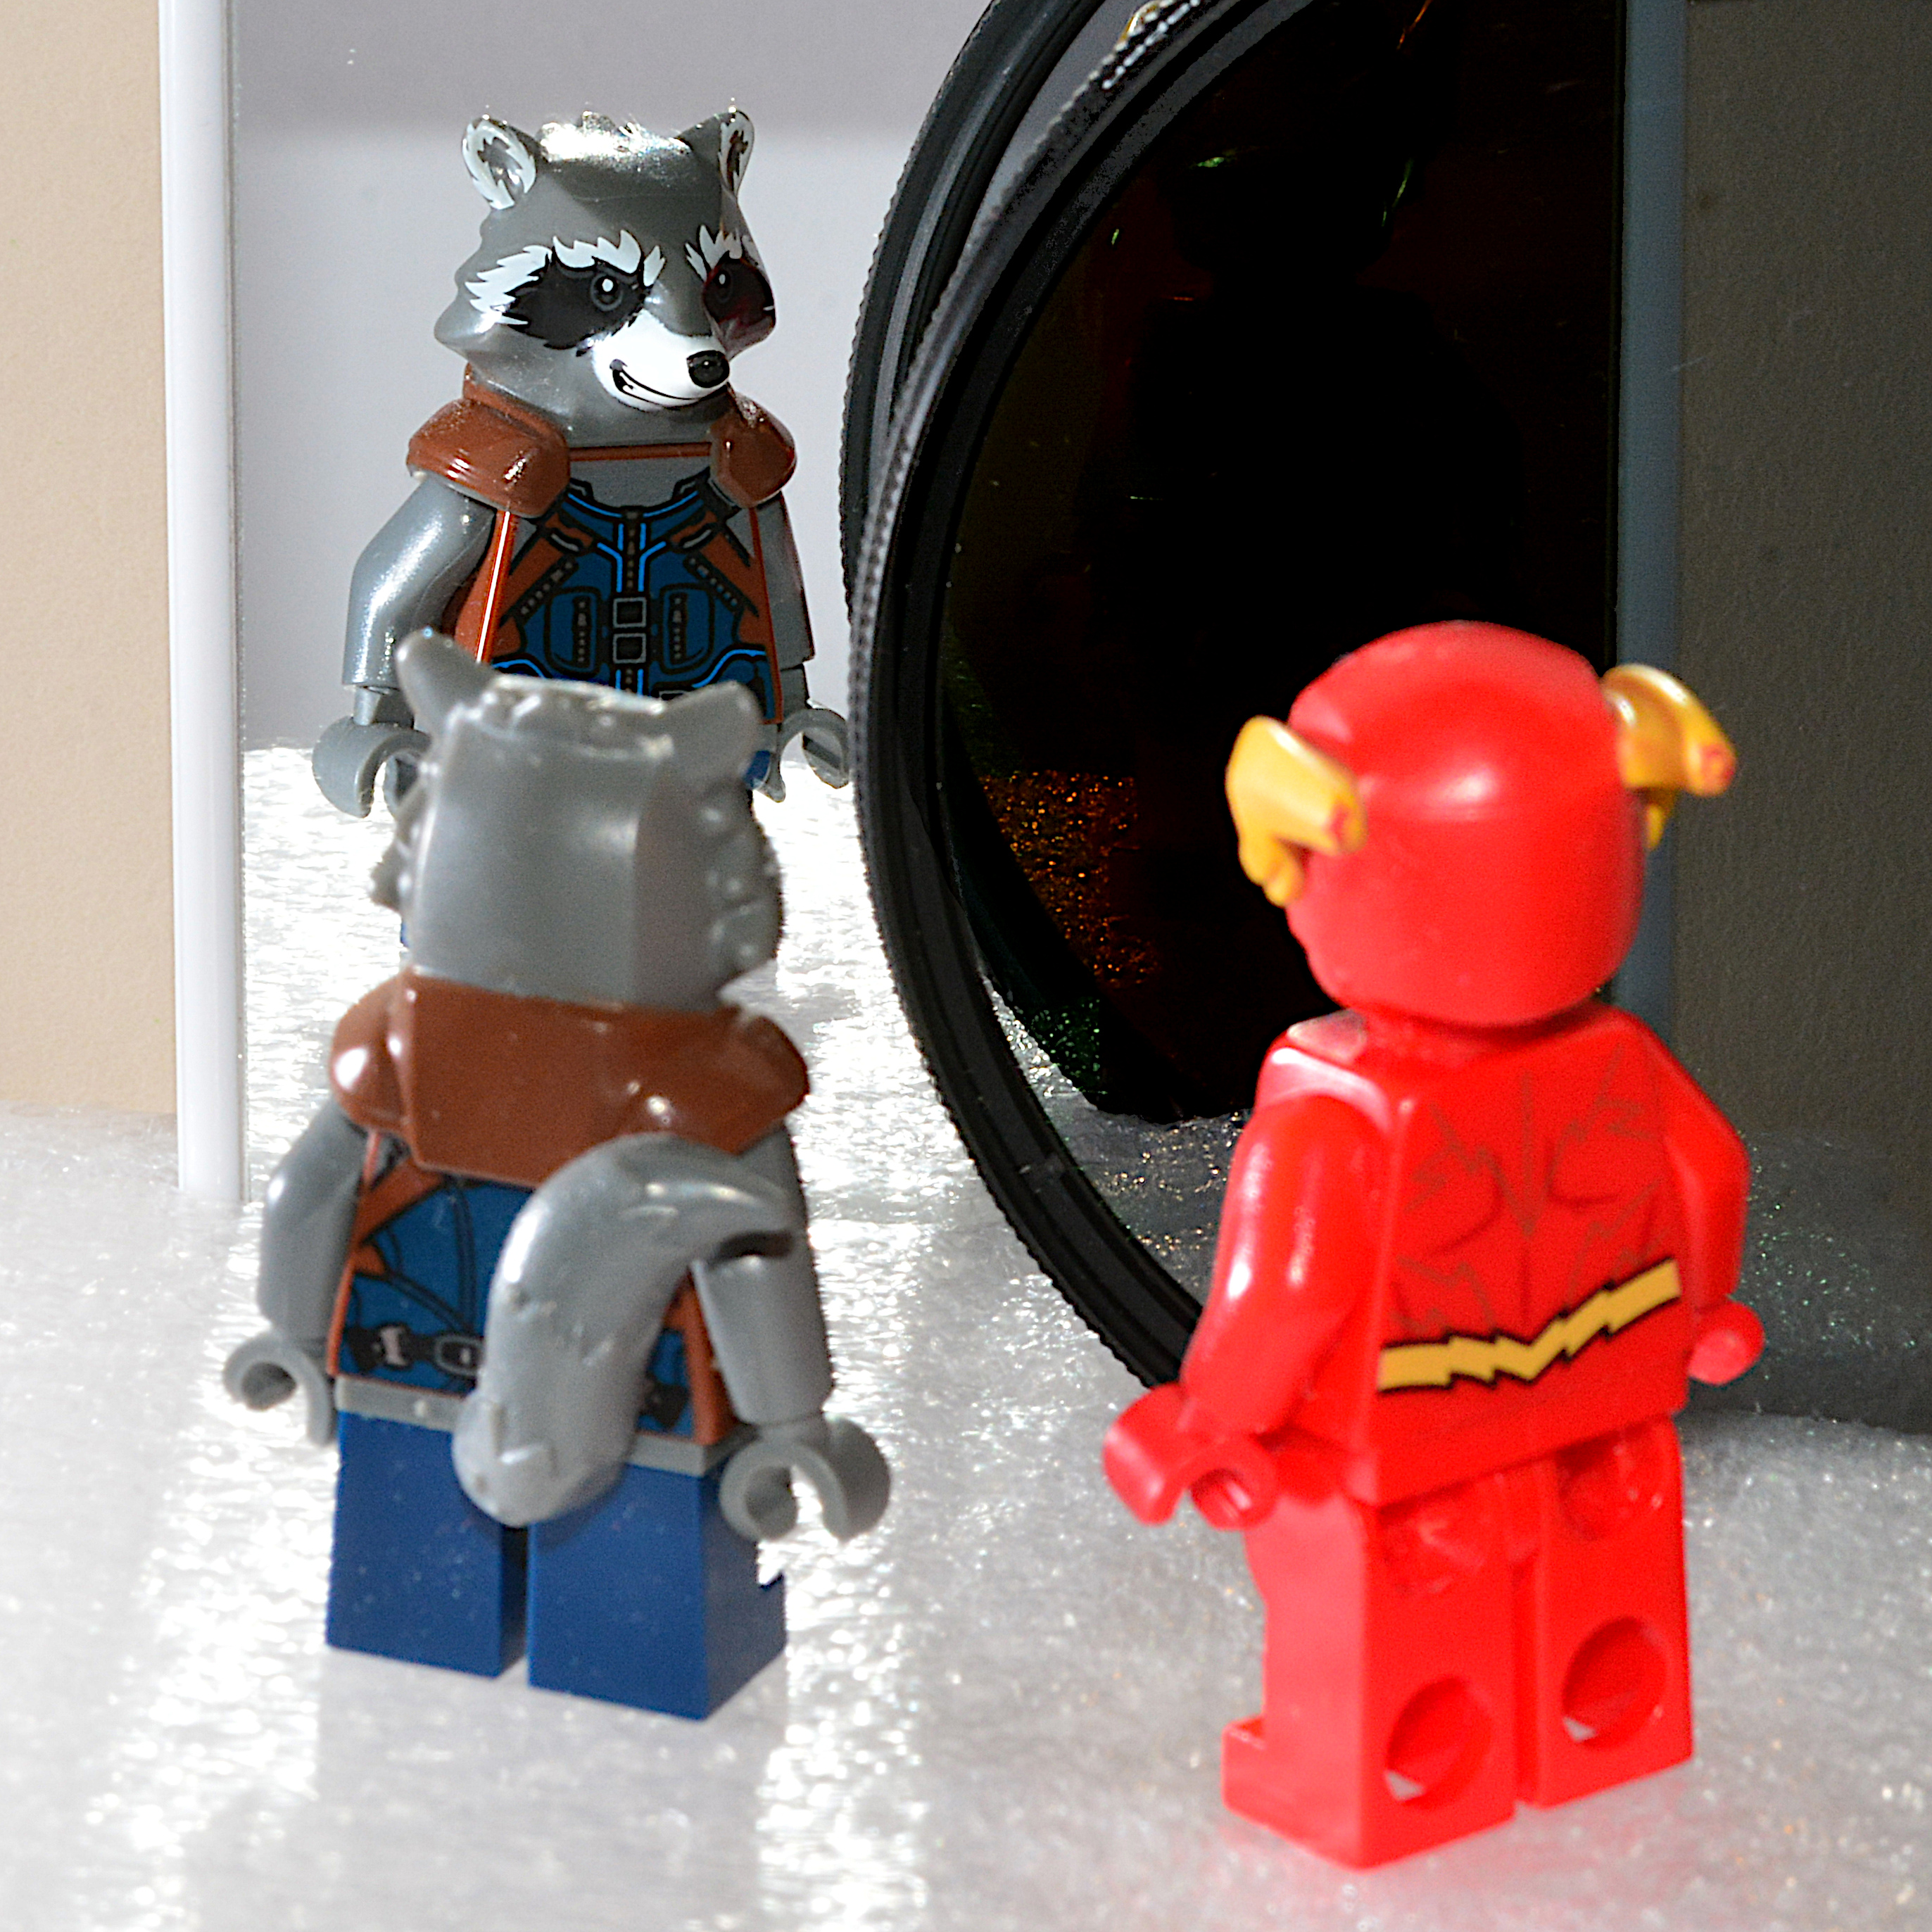
\includegraphics[width=7truecm]{slike/03_circodboj.JPG}
\caption{Linearno polarizirano valovanje pri odboju in prehodu skozi linearni polarizator
vidimo (levo). Cirkularno polarizirano valovanje se pri odboju spremeni iz 
desno polariziranega v levo polarizirano in obratno, zato pri ponovnem 
prehodu skozi cirkularni polarizator slike ni (desno).}
\label{fig:03_CirkularniOdboj}
\end{figure}
\end{example}

\begin{example}{\bf Zamenjava optičnih elementov.}
Poglejmo še učinek vrstnega reda optičnih elementov. Izberimo
kombinacijo linearnega in cirkularnega polarizatorja. V enem primeru postavimo
linearni polarizator pred cirkularnega, v drugem pa za njega. Razlika
v prepuščeni svetlobi jasno kaže pomembnost vrstnega reda optičnih
elementov in seveda tudi vrstnega reda zapisa matrik.
\begin{figure}[h!]
\centering
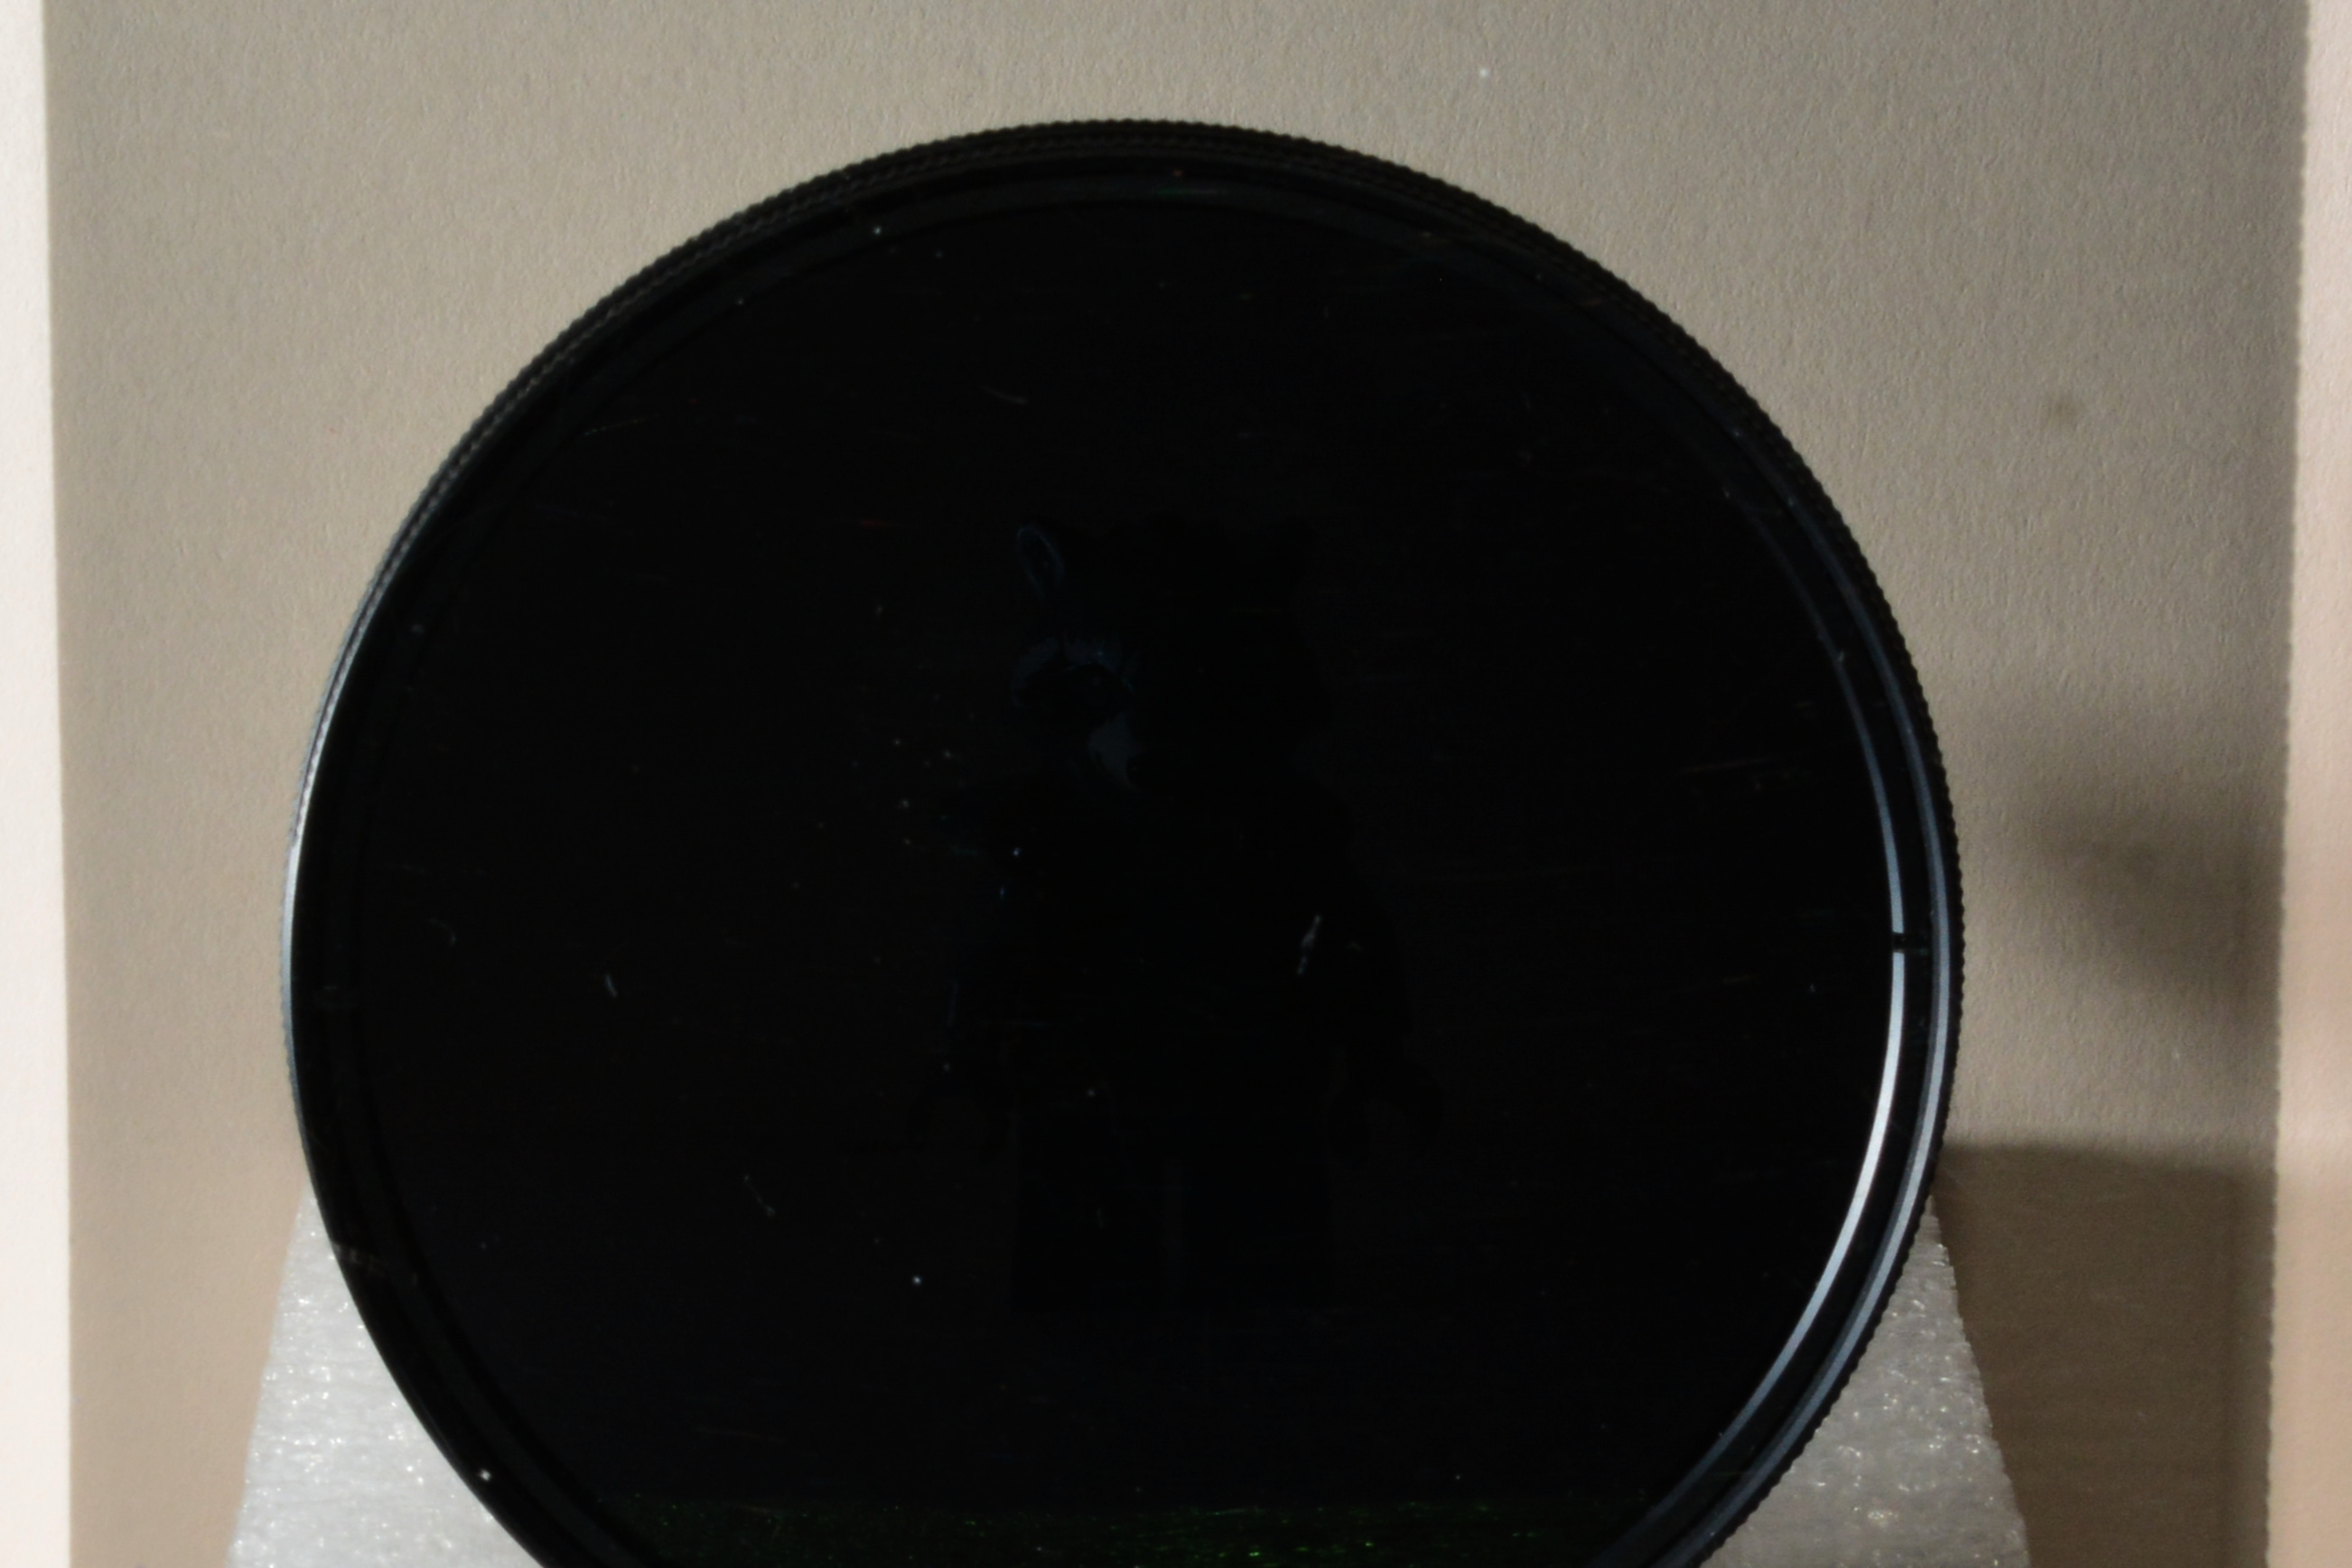
\includegraphics[width=7truecm]{slike/03_vrstnired1.JPG}\hfill
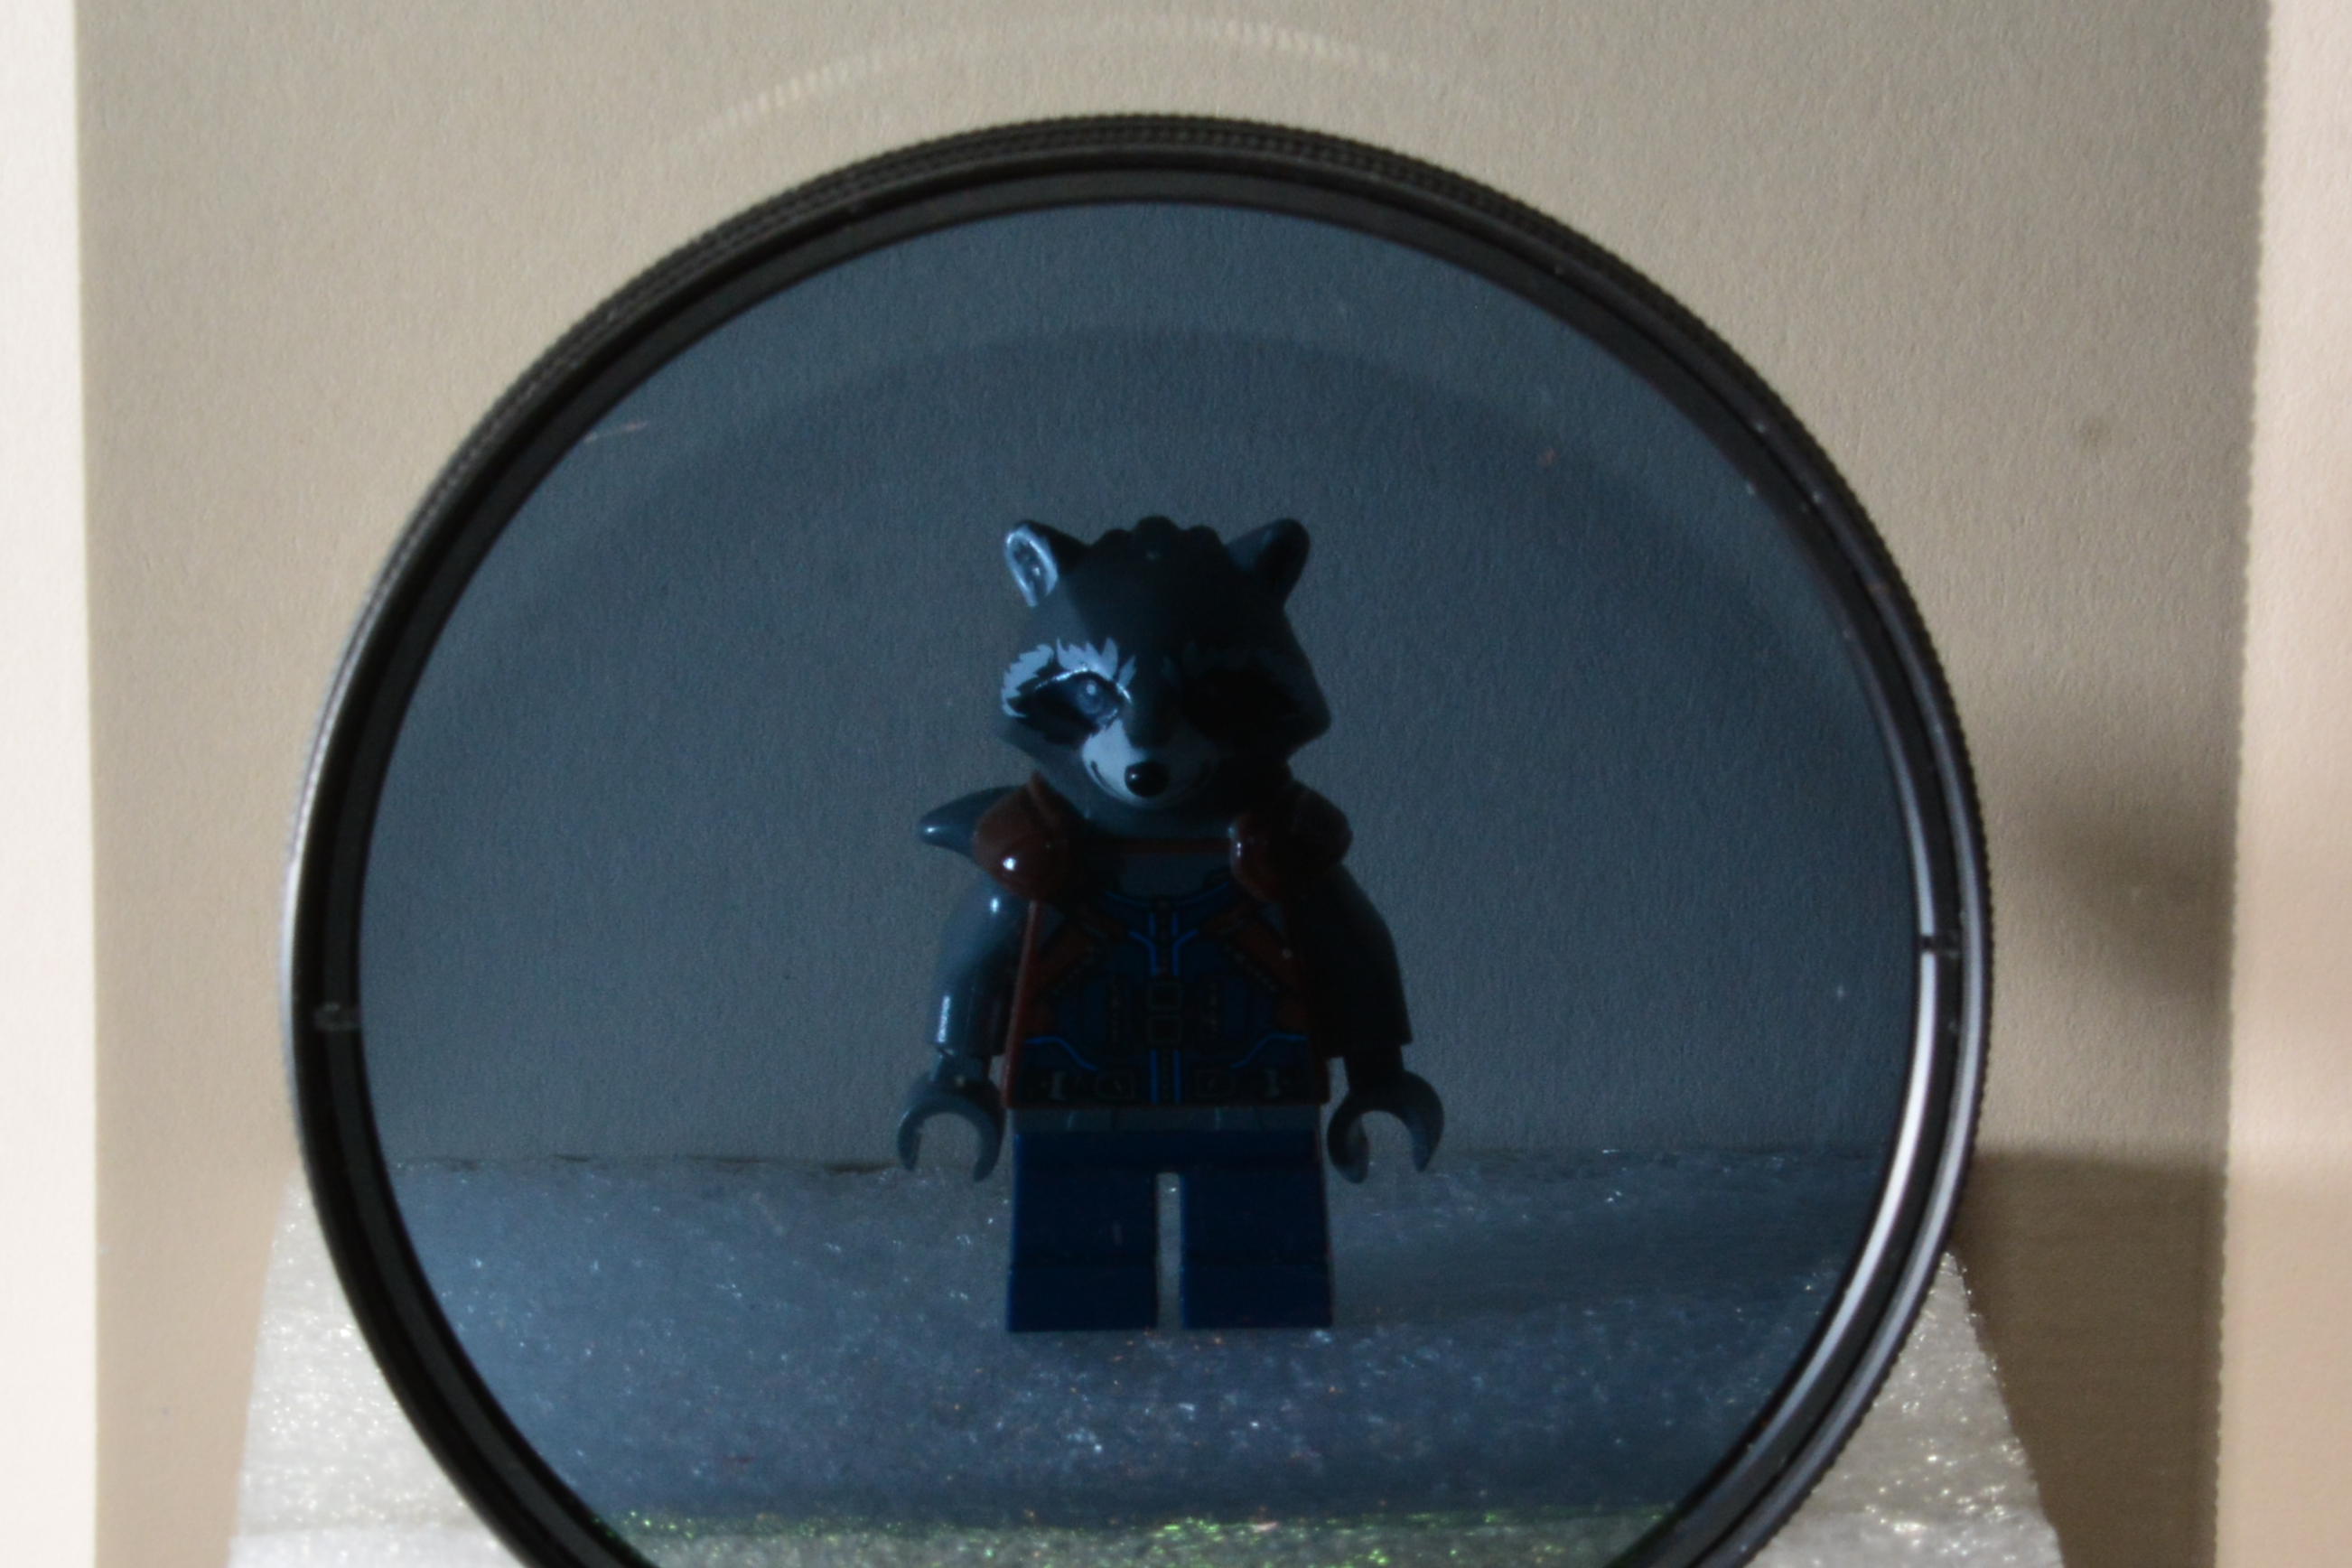
\includegraphics[width=7truecm]{slike/03_vrstnired2.JPG}
\caption{Učinek vpliva vrstnega reda cirkularnega in linearnega polarizatorja.
Na levi sliki je spredaj linearni polarizator in za njim cirkularni, na desni sliki
je vrstni red obrnjen in svetloba je prepuščena.}
\label{fig:03_VrstniRed}
\end{figure}
\end{example}

\section{Valovna enačba v prevodni snovi}
\label{section:35}
Obravnavajmo za konec še valovno enačbo v prevodni snovi. Snov naj
bo homogena, izotropna in nenabita ($\varrho_e = 0$). Izhajamo\index{Valovna enačba!{v prevodniku}|see{Telegrafska enačba}}
iz Maxwellovih enačb (enačbe~\ref{eq:Maxwell1}--\ref{eq:Maxwell4}) in zveze:
\begin{equation}
\mathbf{j}_e = \sigma \mathbf{E},
\label{eq:03_65}
\end{equation}
ki povezuje gostoto električnega toka $\mathbf{j}_e $ in jakost 
električnega polja $\mathbf{E}$. Sorazmernostni faktor, ki predstavlja\index{Električna prevodnost}
električno prevodnost, smo označili s $\sigma$. Tipična vrednost
za kovine je $\sigma > 10^6/\si{\ohm\m}$ in za izolatorje 
$\sigma < 10^{-6}/\si{\ohm\m}$. 
Električne tokove moramo upoštevati pri zapisu Amp\`{e}rovega zakona 
(enačba~\ref{eq:Maxwell1}):
\begin{equation}
\nabla\times\mathbf{H} =\frac{\partial\mathbf{D}}{\partial t}+\mathbf{j}_e = 
\varepsilon \varepsilon_0 \frac{\partial\mathbf{E}}{\partial t}+\sigma \mathbf{E}.
\label{eq:03_66}
\end{equation}
Izhajamo iz Faradayevega zakona (enačba~\ref{eq:Maxwell2}) in na njem izvedemo operacijo rotorja:
\begin{equation}
\nabla \times \left( \nabla \times  \mathbf{E}\right) = -\nabla\times \left(
\frac{\partial \mathbf{B}}{\partial t}\right) = - \mu \mu_0 \frac{\partial }{\partial t}
\left( \nabla \times \mathbf{H}\right)\!\!.
\label{eq:03_67}
\end{equation}
Vstavimo enačbo~(\ref{eq:03_66}) in dobimo:
\begin{equation}
\nabla \times \left( \nabla \times  \mathbf{E}\right) =
 -\mu \mu_0 \frac{\partial }{\partial t}
\left( \varepsilon \varepsilon_0 \frac{\partial\mathbf{E}}{\partial t}\right)-
\mu \mu_0 \frac{\partial }{\partial t}\left(\sigma \mathbf{E} \right)\!\!.
\label{eq:03_671}
\end{equation}
Upoštevamo še enačbo~(\ref{eq:03_02}) in dobimo zvezo:
\boxeq{eq:telegrafska}{
\nabla^2\mathbf{E} =  \mu \mu_0\varepsilon \varepsilon_0 \frac{\partial^2\mathbf{E}}{\partial t^2}
+ \mu \mu_0 \sigma \frac{\partial \mathbf{E}}{\partial t}.
}
Zapisano enačbo imenujemo telegrafska enačba. Podobno izpeljemo tudi telegrafsko enačbo
za gostoto magnetnega polja $\mathbf{B}$.\index{Telegrafska enačba}

Ker v telegrafski enačbi nastopa prvi odvod po času, po analogiji z mehanskimi
sistemi pričakujemo, da se valovanje v snovi duši oziroma slabi (atenuira). 
Rešitev zato iščemo v obliki ravnega valovanja:
\begin{equation}
\mathbf{E}(\mathbf{r},t) = \mathbf{E}_0 e^{i\mathbf{k}\cdot \mathbf{r} - i\omega t},
\label{eq:03_68}
\end{equation}
pri čemer dopuščamo možnost kompleksnega valovnega vektorja,\index{Valovni vektor!kompleksni} katerega imaginarni del
bo opisoval pojemanje amplitude. Ko nastavek (enačba~\ref{eq:03_68})
vstavimo v telegrafsko enačbo (enačba~\ref{eq:telegrafska}), dobimo:
\begin{equation}
-k^2 \mathbf{E} = \mu \mu_0\varepsilon \varepsilon_0 \left (-\omega^2 \mathbf{E}\right)
+ \mu \mu_0 \sigma \left(-i \omega\right)\mathbf{E}.
\label{eq:03_69}
\end{equation}
Sledi:
\begin{equation}
k^2 = \mu \mu_0\varepsilon \varepsilon_0 \omega^2 + i \mu \mu_0 \sigma\omega = 
\frac{\omega^2}{c_0^2} \varepsilon \mu  + i \frac{\omega^2}{c_0^2}\frac{\sigma \mu}{\varepsilon_0\omega}.
\label{eq:03_70}
\end{equation}
Vstavimo valovno število v vakuumu $k_0 = \omega/c_0$ in dobimo:
\begin{equation}
k^2 = k_0^2 \left( \varepsilon \mu + i \frac{\sigma \mu}{\varepsilon_0\omega} 
\right)\!\!.
\label{eq:03_71}
\end{equation}
Vpeljemo kompleksni lomni količnik $\mathcal{N}$, tako da velja:\index{Lomni količnik!kompleksni}
\boxeq{eq:nkompleks}{
k = k_0 \mathcal{N}.
}
Pri tem je:
\boxeq{eq:nkompleks2}{
\mathcal{N}^2 = \varepsilon \mu + i \frac{\sigma \mu}{\varepsilon_0\omega}.
}
Kompleksni lomni količnik $\mathcal{N}$ zapišemo kot vsoto realnega $n'$ in imaginarnega
dela $n''$:
\begin{equation}
\mathcal{N}^2 = (n'+in'')^2 = n'^2 -n''^2 + 2i n'n''.
\label{eq:03_72}
\end{equation}
Označimo realni del $\mathcal{N}^2$ (enačba~\ref{eq:nkompleks2})
z $x = \varepsilon \mu$ in imaginarni del z $y = \sigma \mu/\varepsilon_0\omega$.  
Rešujemo torej enačbo:
\begin{equation}
x + iy = n'^2 -n''^2 + 2i n'n''.
\label{eq:03_72a}
\end{equation}
Ločimo realni del:
\begin{equation}
x = n'^2 -n''^2
\label{eq:03_73}
\end{equation}
in imaginarni del:
\begin{equation}
y = 2n'n''.
\label{eq:03_74}
\end{equation}
Izrazimo $n''$ iz druge enačbe in ga vstavimo v prvo. Dobimo kvadratno enačbo:
\begin{equation}
n'^2-(y/2n')^2 = x
\label{eq:03_75}
\end{equation}
z rešitvijo:
\begin{equation}
n'^2 = \left(x + \sqrt{x^2+y^2}\right)/2.
\label{eq:03_76}
\end{equation}
Pri tem smo se omejili na rešitev s pozitivnim predznakom, saj je negativen predznak
za navadne snovi nesmiseln. Iz enačbe~(\ref{eq:03_73}) izračunamo še imaginarni del, 
ki je enak:
\begin{equation}
n''^2 = \left(-x + \sqrt{x^2+y^2}\right)/2.
\label{eq:03_77}
\end{equation}
Vstavimo izraza za $x$ in $y$ in dobimo:
\begin{equation}
n'^2 = \frac{1}{2}\left(\varepsilon \mu + \sqrt{(\varepsilon \mu)^2 + 
\left(\frac{\sigma \mu}{\varepsilon_0\omega}\right)^2}\right)
\label{eq:03_78}
\end{equation}
in
\begin{equation}
n''^2 = \frac{1}{2}\left(-\varepsilon \mu + \sqrt{(\varepsilon \mu)^2 + 
\left(\frac{\sigma \mu}{\varepsilon_0\omega}\right)^2}\right)\!\!.
\label{eq:03_79}
\end{equation}
Pogosto nas zanimajo nemagnetne snovi, v katerih je $\mu=1$. V takih
snoveh se kvadrat realnega dela lomnega količnika poenostavi v :
\begin{equation}
n'^2 = \frac{1}{2}\left(\varepsilon + \sqrt{\varepsilon^2 + 
\left(\frac{\sigma}{\varepsilon_0\omega}\right)^2}\right)\!\!,
\label{eq:03_80}
\end{equation}
kvadrat imaginarnega dela pa v:
\begin{equation}
n''^2 = \frac{1}{2}\left(-\varepsilon + \sqrt{\varepsilon^2 + 
\left(\frac{\sigma}{\varepsilon_0\omega}\right)^2}\right)\!\!.
\label{eq:03_81}
\end{equation}
Vstavimo zdaj izračunani lomni količnik v nastavek za jakost električnega polja 
(enačba~\ref{eq:03_68}) in poglejmo
primer, ko se svetloba širi v smeri $z$. Dobimo:
\begin{equation}
\mathbf{E} = \mathbf{E}_0 e^{ik_0\mathcal{N}z - i\omega t} = 
\mathbf{E}_0 e^{ik_0 n'z - i\omega t} \cdot e^{-k_0n''z}.
\label{eq:03_82}
\end{equation}
Zadnji člen opisuje eksponentno pojemanje amplitude polja z globino $z$ in ga pogosto
pišemo kot $\exp(-\kappa z)$, pri čemer je $\kappa = k_0 n''$.

V kovinah je prevodnost zelo velika in velja:
\begin{equation}
\frac{\sigma}{\omega\varepsilon_0} \gg \varepsilon.
\label{eq:03_83}
\end{equation}
Potem lahko imaginarni del lomnega količnika zapišemo kot:
\begin{equation}
n'' \approx \sqrt{\frac{\sigma}{2 \omega \varepsilon_0}}.
\label{eq:03_84}
\end{equation}
Parameter $\kappa$ je:
\begin{equation}
\kappa = k_0 n'' = \frac{\omega}{c_0} \sqrt{\frac{\sigma}{2 \omega \varepsilon_0}} = \sqrt{\frac{\mu_0 \omega \sigma}{2}}.
\label{eq:03_85}
\end{equation}
Nazornejše je vpeljati vdorno globino:\index{Vdorna globina}
\begin{equation}
d = \kappa^{-1} = \sqrt{\frac{2}{\mu_0 \omega \sigma}},
\label{eq:03_86}
\end{equation}
ki predstavlja karakteristično globino pojemanja električne poljske jakosti.
V kovinah je zaradi velike prevodnosti vdorna globina zelo majhna. Večina elektromagnetnega
valovanja oziroma izmeničnega toka zato teče po površini prevodnih snovi. Ta pojav poznamo pod imenom
kožni pojav.

\begin{example}{\bf Vdorna globina v bakru.}
Specifična upornost bakra je $\xi = 0,017~\si{\ohm\,\milli\metre^2/\metre}$ in 
prevodnost $\sigma = 1/\xi = 58 \times 10^6/\si{\ohm\metre}$. 
Vdorna globina je odvisna od frekvence elektro\-mag\-net\-nega valovanja, 
zato izračunajmo nekaj primerov: 
\begin{center}
\begin{tabular}{|c|c|}
\hline
$\nu~[\si{Hz}]$ & $d~[\si{nm}]$\\ \hline
50 & $\approx 10~\si{mm}$\\ \hline
$10^6$ & $\approx 100~\si{\micro\metre}$\\ \hline
$10^{10}$ & $\approx 1~\si{\micro\metre}$\\ \hline
$10^{15}$ & $\approx 3~\si{\nano\metre}$\\ \hline
\end{tabular}
\end{center}

Vdorna globina za vidno svetlobo je v bakru torej nekaj nanometrov. 
Izredno kratka vdorna globina v kovinah predstavlja velik problem pri izdelavi prozornih elektrod, 
ki jih potrebujemo na primer za izdelavo sončnih celic
ali tekočekristalnih zaslonov. Zato za ta namen navadno uporabljamo
kovine z razmeroma majhno prevodnostjo (npr. indijev 
kositrov oksid, ITO) in veliko vdorno globino. Debelina plasti, ki
jo nanesemo na steklo in ki še prepušča večino vpadne svetlobe, je 
v takih kovinah razmeroma velika, tipično 
okoli $100~\si{nm}$. 
\end{example}
